\documentclass[a4paper]{report}

%====================== PACKAGES ======================

\usepackage[french]{babel}
\usepackage[utf8x]{inputenc}
%pour gérer les positionnement d'images
\usepackage{float}
\usepackage{amsmath}
\usepackage{graphicx}
\usepackage{url}
%pour les informations sur un document compilé en PDF et les liens externes / internes
\usepackage{hyperref}
%pour la mise en page des tableaux
\usepackage{array}
\usepackage{tabularx}
%pour utiliser \floatbarrier
%\usepackage{placeins}
%\usepackage{floatrow}
%espacement entre les lignes
\usepackage{setspace}
%modifier la mise en page de l'abstract
\usepackage{abstract}
%police et mise en page (marges) du document
\usepackage[T1]{fontenc}
\usepackage[top=2cm, bottom=2cm, left=2.5cm, right=2.5cm]{geometry}
%Pour les galerie d'images
\usepackage{subfig}
\usepackage{titlesec}

%====================== INFORMATION ET REGLES ======================

\hypersetup{							% Information sur le document
pdfauthor = {PALARD Nicolas}
pdftitle = {Stage Master 2 Informatique -
			RealityTech},			% Titre du document
pdfsubject = {Mémoire de Projet},		% Sujet
pdfkeywords = {Research, Augmented Reality, High performance},	% Mots-clefs
pdfstartview={FitH}}					% ajuste la page à la largueur de l'écran
%======================== DEBUT DU DOCUMENT ========================

\begin{document}

%régler l'espacement entre les lignes
\newcommand{\HRule}{\rule{\linewidth}{0.5mm}}

%page de garde
\begin{titlepage}
\begin{center}

% Upper part of the page. The '~' is needed because only works if a paragraph has started.

\includegraphics[width=0.35\textwidth]{./logos/ubx}~\\[1cm]

\textsc{\LARGE Université de Bordeaux - Reality Tech}\\[1.5cm]

\textsc{\Large }\\[0.5cm]

% Title
\HRule \\[0.4cm]

{\huge \bfseries Mémoire de stage\\
				Master 2 Informatique\\
				Image et son\\}

\HRule \\[1.5cm]

% Author and supervisor
\begin{minipage}{0.4\textwidth}
\begin{flushleft} \large
\emph{Auteur:}\\
Nicolas \textsc{PALARD}\\
\end{flushleft}
\end{minipage}
\begin{minipage}{0.4\textwidth}
\begin{flushright} \large
\emph{Client:} \\
Jérémy \textsc{Laviole}\\
\emph{Référent:} \\
Vincent \textsc{LEPETIT}
\end{flushright}
\end{minipage}

\vfill


\includegraphics[width=0.22\textwidth]{./logos/logo-rt-notext}~\\[1cm]
% Bottom of the page
{\large \today}

\end{center}
\end{titlepage}

%page blanche
\newpage
~
%ne pas numéroter cette page
\thispagestyle{empty}
\newpage

\renewcommand{\abstractnamefont}{\normalfont\Large\bfseries}
%\renewcommand{\abstracttextfont}{\normalfont\Huge}

\begin{abstract}
\hskip7mm

\begin{spacing}{1.3}

Dans le cadre de mon stage de fin d'étude, j'ai eu l'occasion de travailler chez \texttt{RealityTech}, une jeune startup dans le domaine de la réalité augmentée spatiale. Durant le temps que j'y ai passé, il m'a été demandé d'étudier les objectifs, les intérêts et les apports de cette technologie. J'ai tout d'abord pu l'apprivoiser par le biais de \texttt{PapARt}, le système de projection interactif que développe la société, avec lequel j'ai développé mes premières applications. Tout au long de ces développements, j'ai découvert les enjeux mais aussi les difficultés inhérentes à de tels systèmes. Ces diverses difficultés ainsi que la rigidité de \texttt{PapARt} m'ont amené à développer un prototype d'une nouvelle plateforme pour la société, dont le but était d'offrir de meilleures performances et d'être plus robuste que le système actuel, tout en en conservant les fonctionnalités. De l'optimisation matérielle à la refonte complète de l'architecture, en passant par l'optimisation algorithmique, il m'a été demandé d'opérer sur tous les fronts afin de créer un prototype viable. Un prototype n'allant pas sans tests, j'ai du m'atteler à réaliser une batterie de tests de performance qui ont permis de mettre en lumière les avancées mais aussi les défauts de ce dernier. Les performances n'étant pas le seul critère de validation du prototype, j'ai poursuivi mon stage en développant un module Unity permettant de le mettre à profit. En plus de permettre l'évaluation de l'utilisabilité du prototype, le module devait aussi fournir aux utilisateurs développeurs de \texttt{RealityTech} la possibilité de créer des applications de réalité augmentée spatiale en résolvant, pour ces derniers, les nombreuses problématiques liées au domaine. Ainsi, pour terminer mon stage, j'ai endossé le costume de l'utilisateur développeur et ai réalisé une application de démonstration en utilisant le module nouvellement créé afin d'en réaliser l'évaluation.\\

\textit{Mot-clés:} Réalité augmentée, réalité augmentée spatiale, interface tangible, programmation haute performance, microservices, unity, processing, vision par ordinateur.

\end{spacing}
\end{abstract}


\tableofcontents
\thispagestyle{empty}
\setcounter{page}{0}
%ne pas numéroter le sommaire

\newpage

%espacement entre les lignes d'un tableau
\renewcommand{\arraystretch}{1.5}

%removing Chapter name and number
\titleformat{\chapter}[display]
  {\normalfont\bfseries}{}{0pt}{\Huge}

%====================== INCLUSION DES PARTIES ======================

~
\thispagestyle{empty}
%recommencer la numérotation des pages à "1"
\setcounter{page}{0}
\newpage

\chapter{Introduction}

Ce mémoire retracera les missions réalisées durant mon stage de Master 2 Informatique pour l'Image et le Son à l'Université de Bordeaux 1 effectué entre Avril et Septembre 2018 (6 mois) dans la société RealityTech. Ce rapport ne couvrira cependant que les 5 premiers mois du stage car la date de rendu de ce dernier précède d'un moi la date de fin du stage.

Le stage a donc été effectué chez RealityTech une jeune start-up de réalité augmentée spatiale. Issue de l'Inria de Bordeaux, l'institut national de la recherche en information et en automatique, cette dernière est la continuité d'un projet de recherche mené par Jérémy Laviole, ex ingénieur de recherche à l'Inria. PapARt\footnote{https://project.inria.fr/papart/fr/}. Paper Augmented Reality ToolKit est un kit de développement (SDK) permettant de créer des expériences de réalité augmentée sous forme d'applications de projection interactive dans des feuilles de papier. Les travaux actuellement effectués a RealityTech visent à améliorer et étendre ce système de projection. Le but est de pouvoir créer, via ce que propose la société, des expériences collaboratives où les objets physiques se mêlent parfaitement au monde numérique que ce soit en créant des interactions avec ceux ci, ou en leur rajoutant du contexte.

Actuellement, RealityTech se développe dans un incubateur de start-up appelé \texttt{La Banquiz}\footnote{http://labanquiz.com} situé 4 rue Eugène et Marc Dulout, a Pessac Centre. L'objectif de La Banquiz est de promouvoir des start-up Open Source\footnote{https://fr.wikipedia.org/wiki/Open\_source} et innovantes en leur apportant des formations, du coaching individuel et collectif, de l'aide pour la recherche de financement et tout ce qui gravite autour de l'accompagnement de jeunes entreprises.

A ce jour RealityTech ne travail qu'avec des laboratoire de recherche (comme ...) et cherche a étendre son secteur d'activité. Les systèmes proposés par la société fournissent les résultats espérés et la dynamique de celle ci s'oriente donc vers une commercialisation du produit. %Parler du fort besoin d'innovation logiciel (plateform haute performance, haut de gamme moyen de gamme bas de game. Expliquer le besoin de démo, de prototype, le salon qu'on a effecuté etc...
% Biblio : PapARt, Inria, Reality Tech, Realité Augmentée Spatiale

\section{Cadre et contexte}
\label{sec:contexte}
RealityTech fait actuellement partie de La Banquizz, un incubateur de startup situé a Pessac Centre.
% Expliquer le cadre de travail, incubateur, beaucoup de réunion, de démarchage, besoin d'applications de démonstration, besoin de prototype pour avoir des fonds etc autonomie très importante ..
% Parler du contexte  en terme de logiciel : volonté d'évolué et de partir vers une nouvelle base moins contraignante que celle présente actuellement + volonté d'ouverture au grand public (ce qui a fait que j'ai du dev unity) + modularité
% Peut être parler plus en détail de PapARt (calibration camera projecteur, expliqué qu'on travail avec des caméra, a l'échelle dans le monde réel (beaucoup de problèmes de calibration etc ...)

\begin{center}
Problématique du sujet
\end{center}


\section{Objectifs}
Le déroulement du stage a été fortement guidé par les besoins de la société.
\paragraph{Applications de démonstration}Le premier gros objectif du stage était le développement d'applications de démonstration en utilisant le produit de l'entreprise. Le but était de comprendre l'essence, le fonctionnement global du produit et ce qu'il était possible/impossible de réaliser avec celui ci. Cet objectif m'a permis d'acquérir à la fois une vision globale de l'architecture logiciel et du fonctionnement interne du kit de développement, et de l'architecture matérielle nécessaire a l'utilisation du kit. En développant ces applications de démonstration, j'ai acquis une vision globale du projet qui m'a permis d'avoir une certaine autonomie assez rapidement

\paragraph{Plateforme haute performance} Le deuxième objectif était de réaliser une preuve de concept haute performance du produit. En effet, comme je l'ai expliqué dans la partie sur le contexte (voir ~\ref{sec:contexte}), l'entreprise se lançait dans le développement d'une nouvelle plateforme haute performance.
% TODO pas fini

\paragraph{Kit de développement} Le dernière objectif était le développement d'un nouveau kit de développement pour Unity3D.  % TODO expliciter

\newpage
\chapter{Notions}
\label{chap:notions}

Le domaine d'activité qui entoure ce stage est très riche en termes de notions et de vocabulaire. Afin de mieux comprendre de quoi il va être question tout au long de ce rapport, il est nécessaire d'en définir les notions de base.

\paragraph{Réalité virtuelle}
La réalité virtuelle plus communément appelé \emph{Virtual Reality (VR)} désigne l'ensemble des environnements purement numériques (fig~\ref{fig:realityspectrum}), qu'ils soient réalistes ou non, dans lesquels aucune interaction avec l'environnement réel n'est possible et inversement. Cette réalité se base très généralement sur un casque \emph{Head Mounted Display (HMD)} dont l'utilisateur doit se munir afin d'être immergé dans un monde numérique avec lequel il peut interagir. Dans la réalité virtuelle, l'immersion est une notion importe lorsqu'il s'agit de la différenciée d'un simple programme informatique.

\begin{figure}[H]
\centering
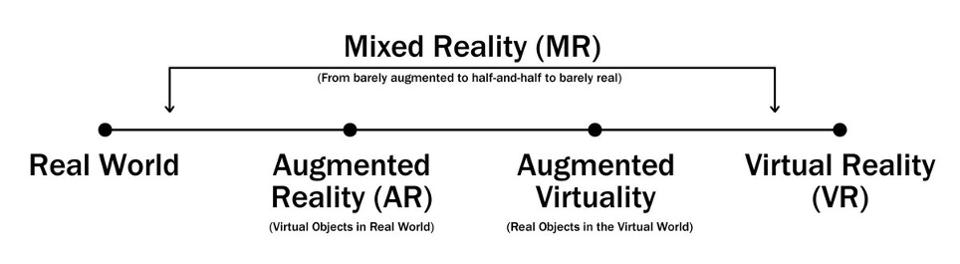
\includegraphics[width=\linewidth]{images/RealitySpectrum}
\caption{Représentation de continuum de la virtualité par Milgram et Kishino, 1995\cite{milgram1995augmented}}
\label{fig:realityspectrum}
\end{figure}

\paragraph{Réalité augmentée}
La réalité augmentée plus communément appelé \emph{Augmented Reality (AR)} quant a elle est un sous domaine de la réalité virtuelle. L'idée de la réalité augmentée est de venir superposer à l'environnement réel des éléments virtuels. Ces éléments vont alors venir "augmenter" notre monde en apportant le plus souvent des compléments d'informations. Elle est donc qualifié de sous domaine de la réalité virtuelle car l'utilisateur n'est plus immergé dans un environnement complètement numérique mais du contenu virtuel est ajouté en contexte à la vision réelle. Par abus de langage le terme de réalité augmentée est souvent utilisé pour parler de réalité mixte dont la notion est détaillé dans cette partie.
Il faut noter que ce type de réalité ne se base pas uniquement sur des \emph{HMD} mais peut être aussi apprécié à l'aide d'un téléphone par exemple (fig~\ref{fig:AR}).

\begin{figure}[H]
\centering
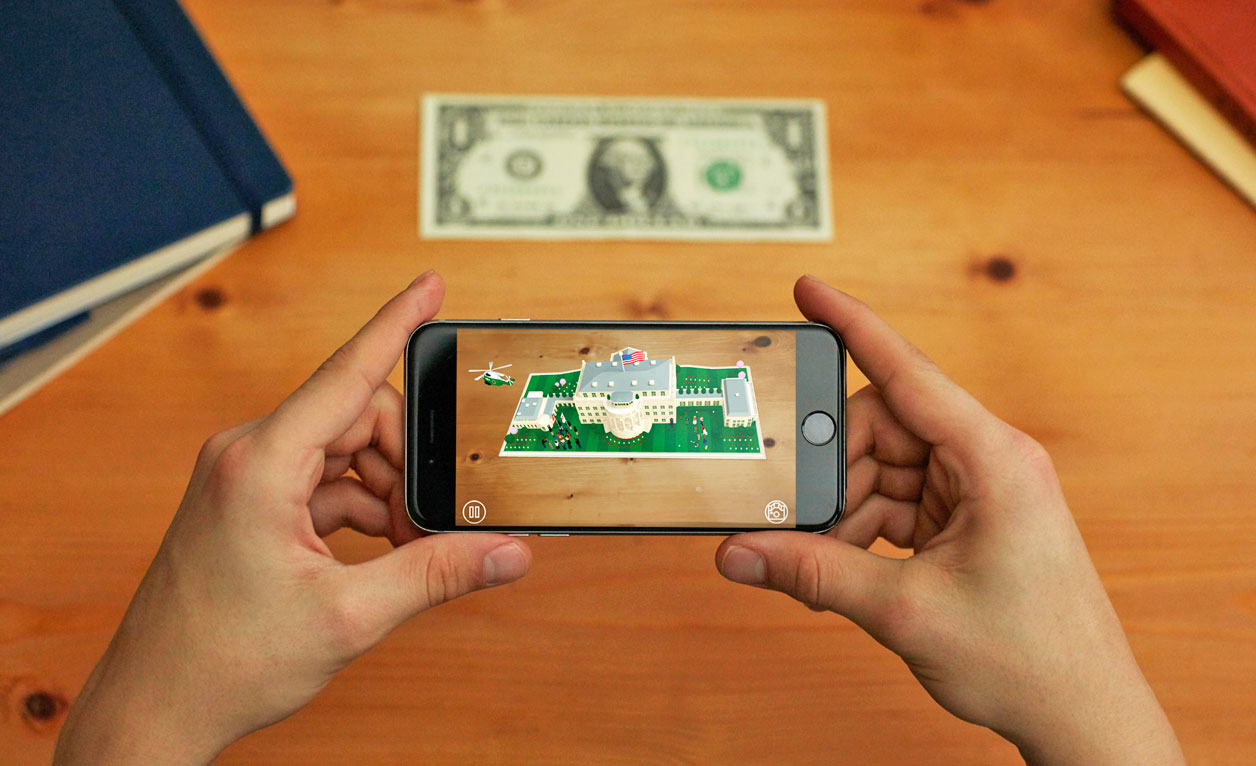
\includegraphics[width=0.55\textwidth]{images/AR}
\caption{Réalité augmentée vu au travers d'un téléphone\protect\footnotemark}\label{fig:AR}
\end{figure}
\footnotetext{Source: \href{https://www.engadget.com}{https://www.engadget.com}}

\paragraph{Réalité mixte}
La réalité mixte, ou hybride, plus communément appelé \emph{Mixed Reality (MR)}, ou \emph{Crossed Reality (XR)}, est la fusion parfaite de l'environnement numérique et de l'environnement physique (fig~\ref{fig:realityspectrum}). Dans ce "nouvel" environnement, les objets physiques et numériques coexistent et peuvent interagir entre eux et par exemple une table peut devenir une plateforme pour un personnage virtuel (fig~\ref{fig:youngconker}). Souvent confondu avec la réalité augmentée, cette dernière se différencie car elle ne propose pas seulement une visualisation des objets numériques, elle propose aussi des méthodes d'interactions avec ce contenu et c'est cette notion d'interaction qui permet de la différencier. A l'heure actuelle la réalité mixte nécessite un dispositif de type \emph{HMD} pour être appréciée comme par exemple  l'\texttt{HoloLens} de \texttt{Microsoft}.

\begin{figure}[H]
\centering
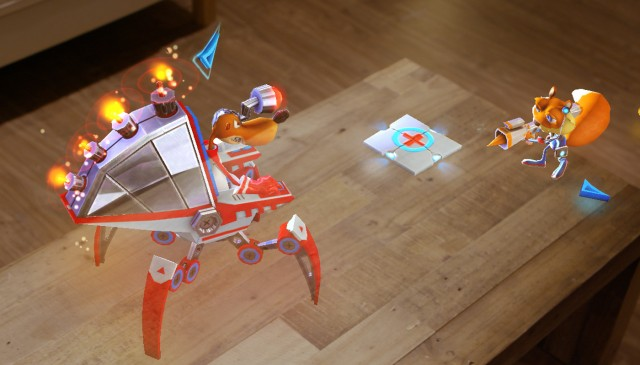
\includegraphics[scale=0.4]{images/youngconker}
\caption{Asobo Studio\texttrademark - Young Conker\copyright}
\label{fig:youngconker}
\end{figure}

\paragraph{Réalité augmentée vue au travers}
% Trouver qui l'a inventé et quand
La réalité augmentée vue au travers, plus communément appelé \emph{See Through Augmented Reality (STAR)} est une technique de visualisation de la réalité augmentée ou les éléments numériques sont vu au travers d'un écran (fig~\ref{sub:STARGO}) ou d'un \emph{HMD} (fig~\ref{sub:STARHolo}). C'est le type de visualisation le plus  utilisé actuellement. L'un des défauts majeur de ce type de visualisation est que la plus part du temps, chaque utilisateur a besoin de son propre écran ou casque pour pouvoir en profiter pleinement ce qui limite grandement les expériences collaboratives. Aussi les principaux défauts liés aux écrans s'appliquent aussi, a savoir fatigue visuel etc.  

\begin{figure}[H]
    \centering
	\subfloat[Pokémon GO - Vue au travers téléphone\protect\footnotemark]{
      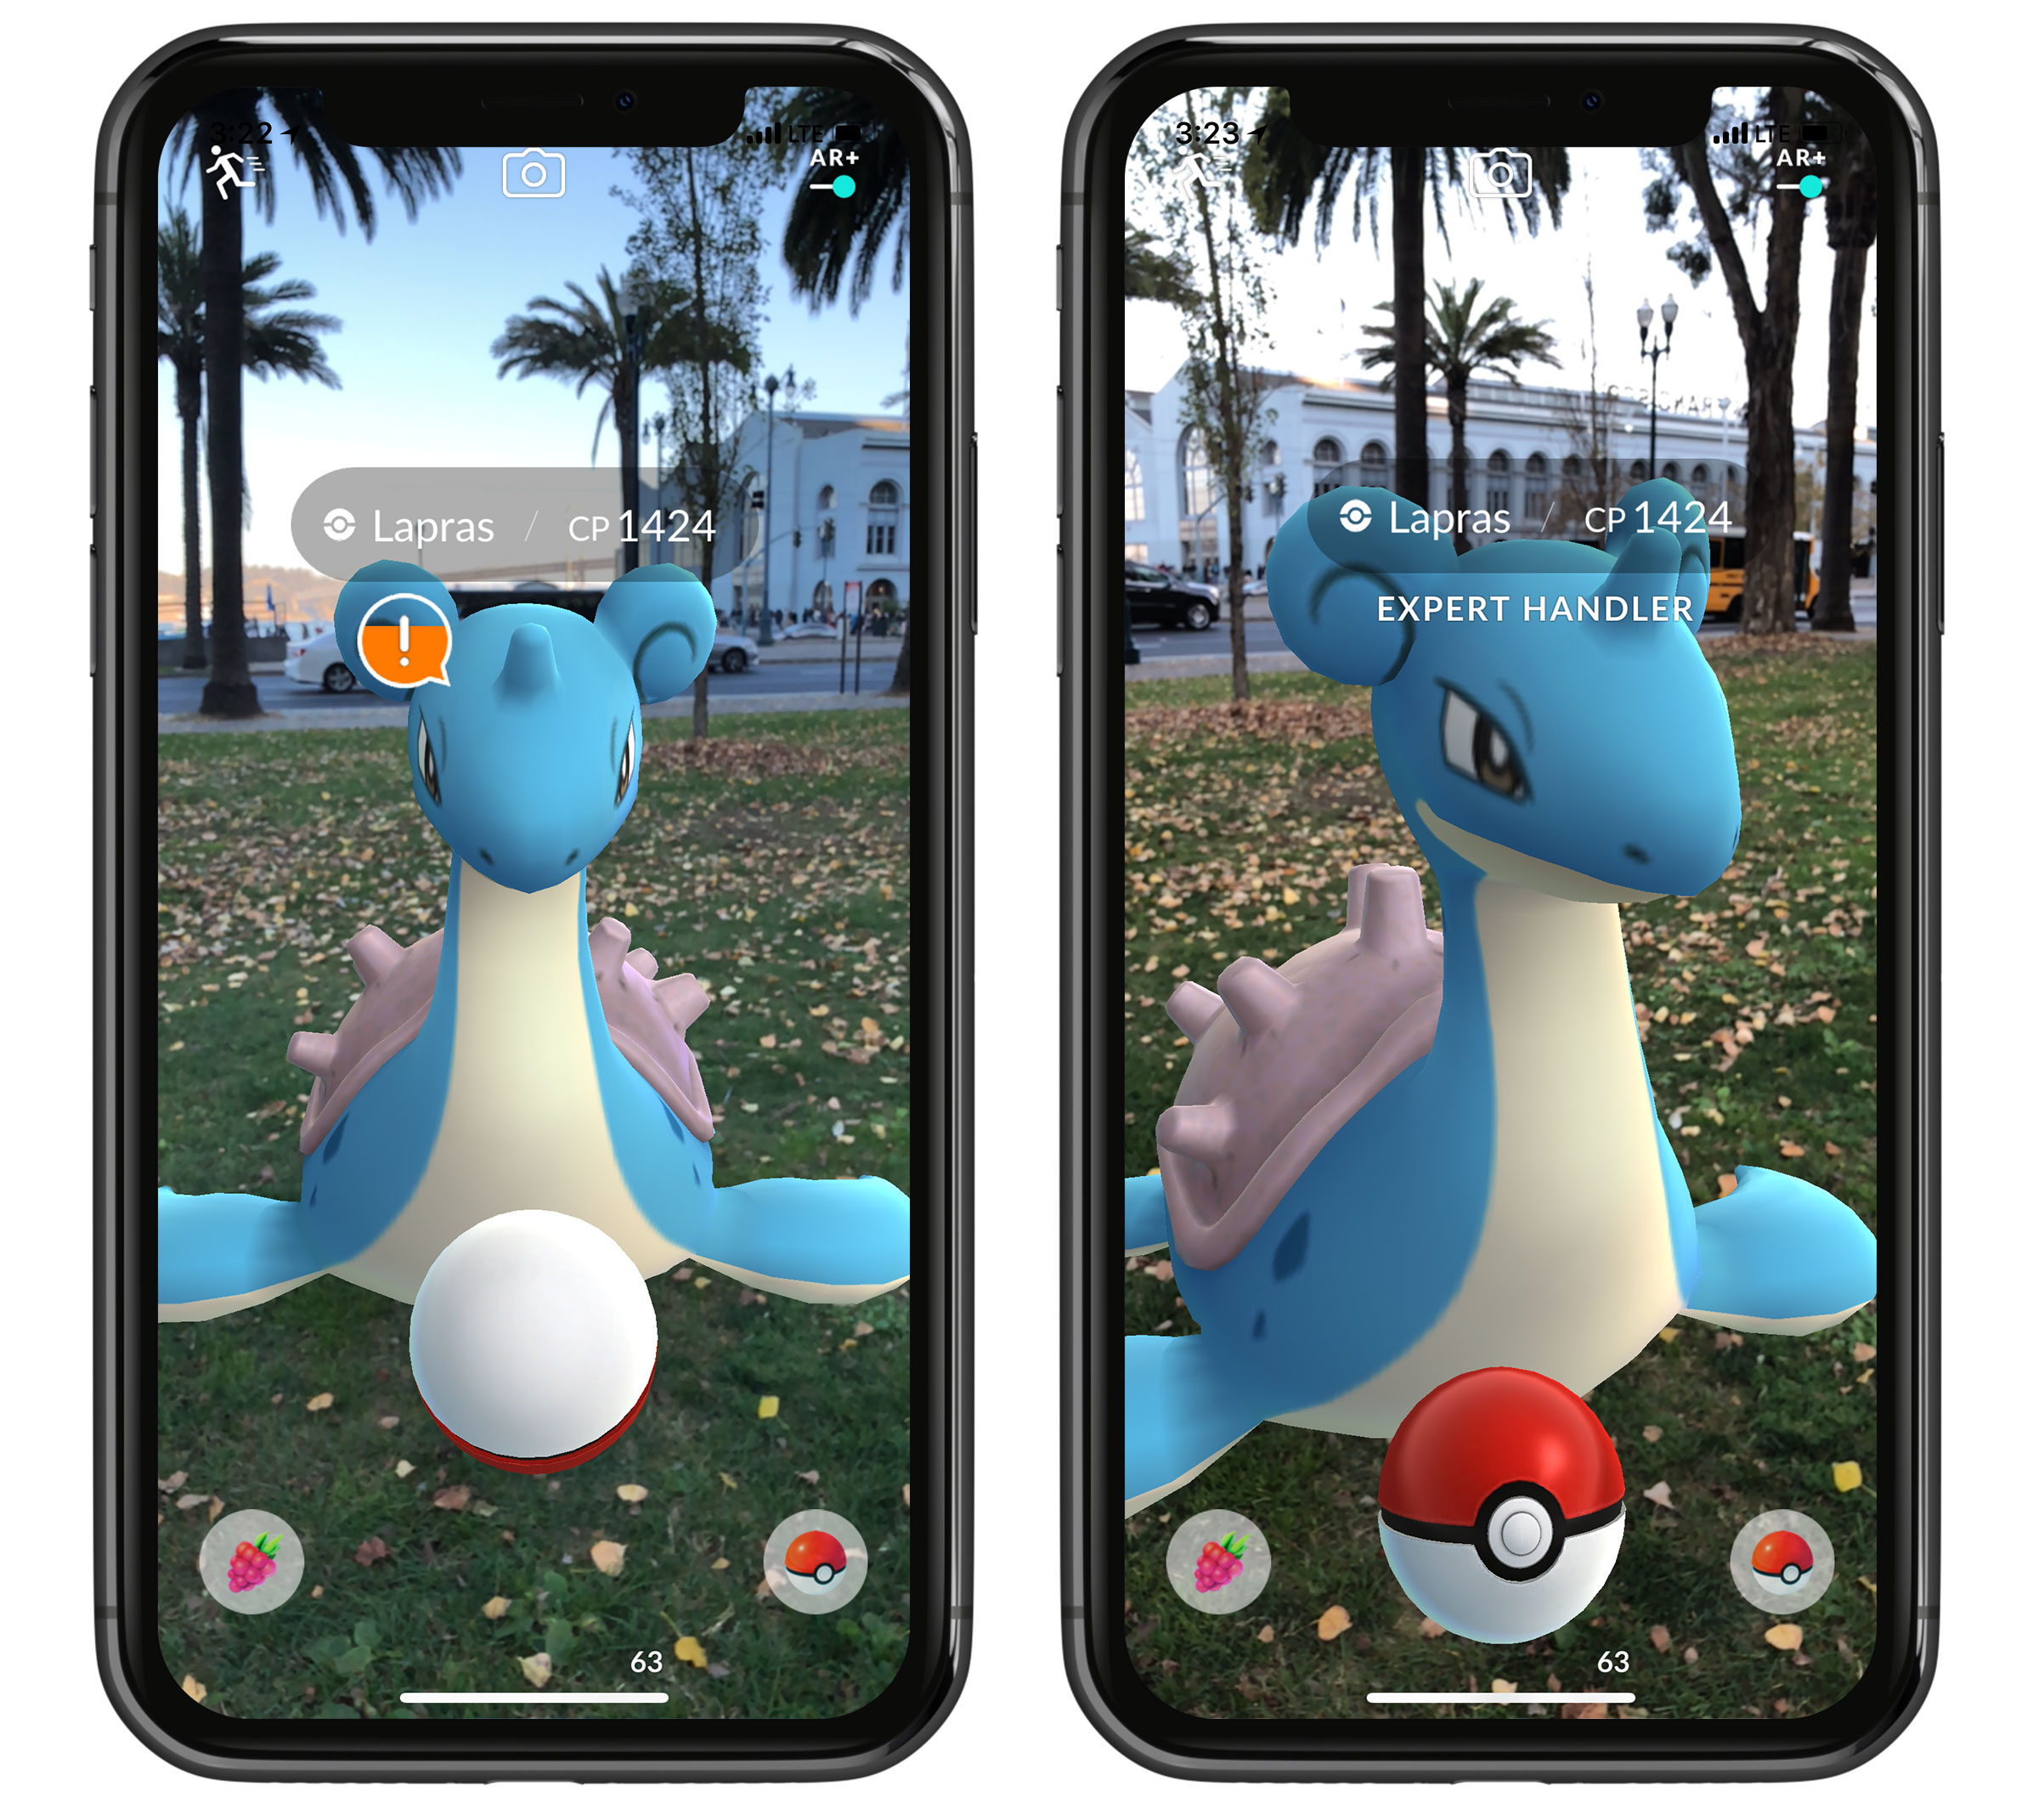
\includegraphics[width=0.45\textwidth]{images/pokemongo}
      \label{sub:STARGO}
      }
    \subfloat[Microsoft HoloLens - Vue au travers casque\protect\footnotemark]{
      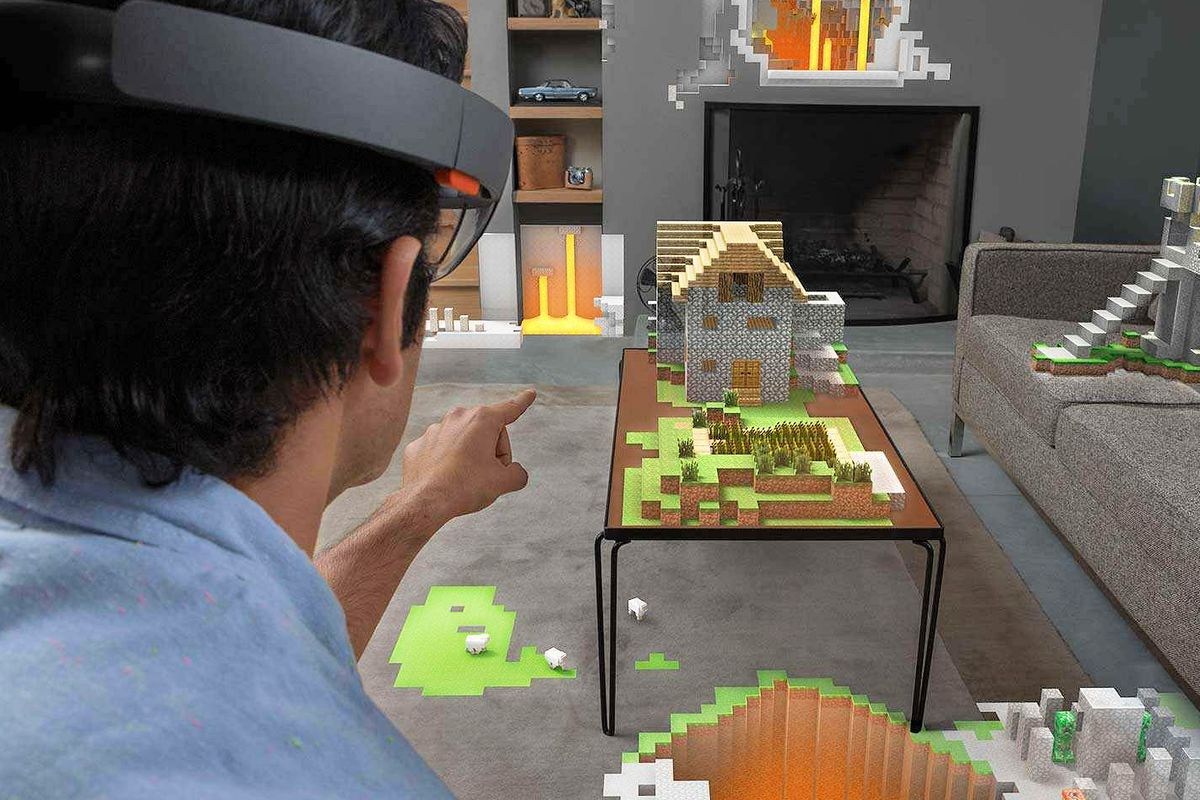
\includegraphics[width=0.45\textwidth]{images/hololens}
      \label{sub:STARHolo}
      }
\caption{Réalité augmentée vue au travers}
\label{fig:STAR}
\end{figure}
\footnotetext{Source: \href{https://pokemongolive.com/fr/}{Pokemon GO}}
\footnotetext{Source: \href{https://www.microsoft.com/fr-fr/hololens}{Microsoft HoloLens}}

\paragraph{Réalité augmentée spatiale}
% Trouver qui l'a inventé et quand
La réalité augmentée spatiale, plus communément appelé \emph{Spatial Augmented Reality (SAR)} est une technique de visualisation de la réalité augmentée se basant sur un dispositif de projection. Les éléments virtuels qui viennent "augmenter" le monde réel sont alors projetés dans l'espace (fig~\ref{fig:SAR}), d'où le terme spatiale. Cette notion d'augmentation de l'espace tend à rendre cette technologie naturellement collaborative car les projections ne dépendent pas d'un dispositif visuel personnel et sont obligatoirement partagées. La SAR permet aussi de favoriser le développement d'interface tangible, en effet, la visualisation se faisant directement sur les objets physiques, la tendance à développer des interfaces en communion avec ceux ci est très forte car très naturel.

\begin{figure}[H]
\centering
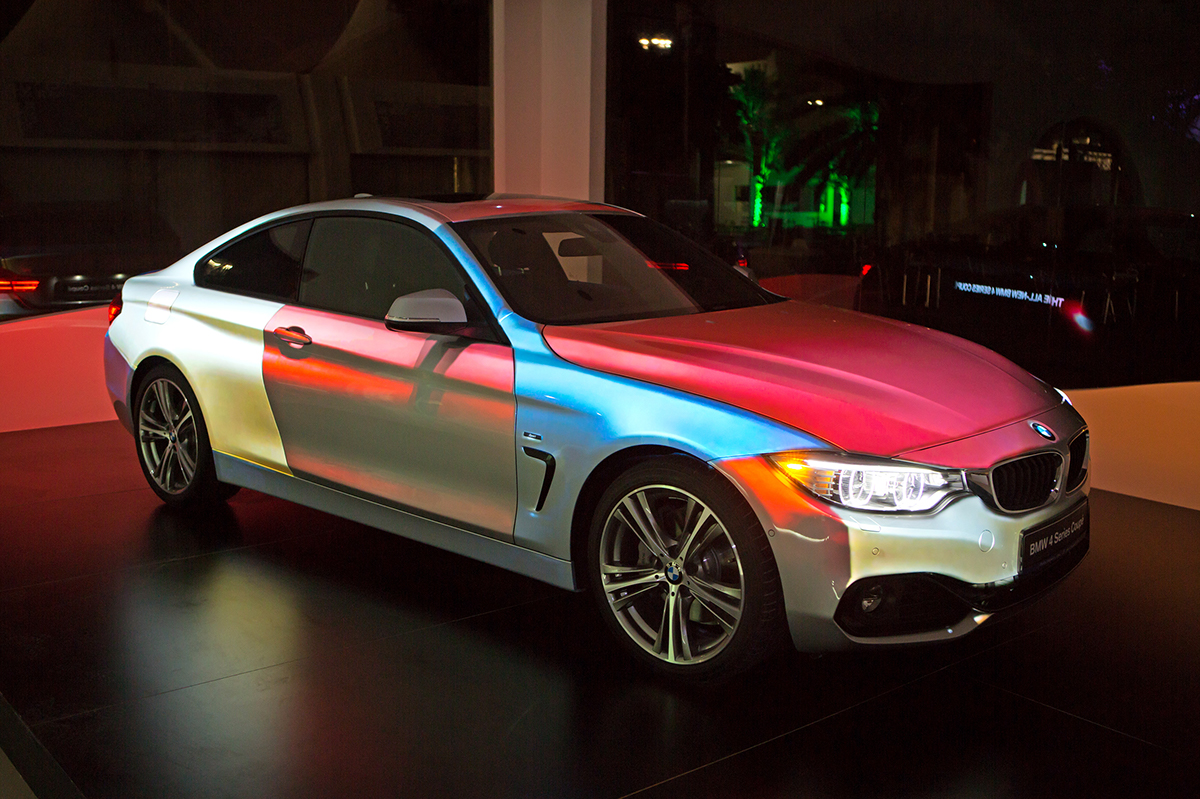
\includegraphics[width=0.5\textwidth]{images/SARMappingCar2}
\caption{Présentation d'une voiture en utilisant de la réalité augmentée spatiale\protect\footnotemark}
\label{fig:SAR}
\end{figure}
\footnotetext{Source: {Google Image}}

\paragraph{Interface tangible}
Une interface utilisateur tangible ou \emph{Tangible User Interface (TUI)} est une interface utilisateur via laquelle des objets physiques, ou encore le toucher, permettent de manipuler des données numériques (fig~\ref{sub:TUI}). Les interfaces utilisateurs tangibles remplacent très souvent les interfaces utilisateur graphiques (fig~\ref{sub:GUI}) où \emph{Graphical User Interface (GUI)} dans la plupart des application de réalité augmentée car elles fournissent un contrôle direct à l'utilisateur sur ce qu'il souhaite manipuler (par opposition au contrôle indirect, comme la souris, nécessaire à la manipulation des GUI).

\begin{figure}[H]
    \centering
	\subfloat[Interface Utilisateur Graphique (GUI)\protect\footnotemark]{
      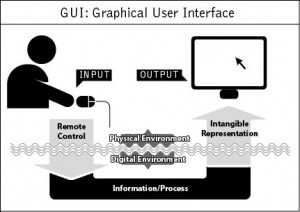
\includegraphics[width=0.45\textwidth]{images/GUI}
      \label{sub:GUI}
      }
    \subfloat[Interface Utilisateur Tangible (TUI)\protect\footnotemark]{
      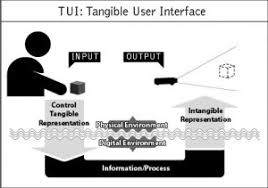
\includegraphics[width=0.45\textwidth]{images/TUI}
      \label{sub:TUI}
      }
\caption{Différences des interfaces utilisateurs}
\label{fig:GUITUI}
\end{figure}
\footnotetext{Source: \href{http://iconlibrary.iconshock.com/design/from-gui-to-tui/}{Icon Library - From GUI to TUI}}
\footnotetext{Source: \href{http://iconlibrary.iconshock.com/design/from-gui-to-tui/}{Icon Library - From GUI to TUI}}

\paragraph{Calcul haute performance}
Le calcul haute performance ou \emph{General-Purpose computing on Graphics Processing Units (GPGPU)} désigne une méthode de calcul utilisant la carte graphique (GPU) plutôt que le processeur (CPU). Cette technique permet de bénéficier de la puissance de la carte graphique afin de réaliser du calcul en parallèle et est très souvent utilisée pour la plupart des traitement lourd comme par exemple le rendu d'une scène 3D, l'encodage de vidéo, les simulations physiques (particules) etc. Cette technique repose sur le grand nombre de cœurs présent dans les cartes graphiques (contrairement aux processeurs) et sur la capacité de chacun de ces cœurs à effectué des opérations simples de manière très efficace. Le calcul haute performance ne peut cependant pas ce passer du CPU qui va être principalement utilisé pour récolter et transférer les données traités ou à traiter.
% Expliquer comment ca marche (carte graphique beaucoup de coeur pour faire des opérations simple, CPU pas beaucoup de coeur donc plus lent)
% Ajouter image comparaison

\begin{figure}[H]
\centering
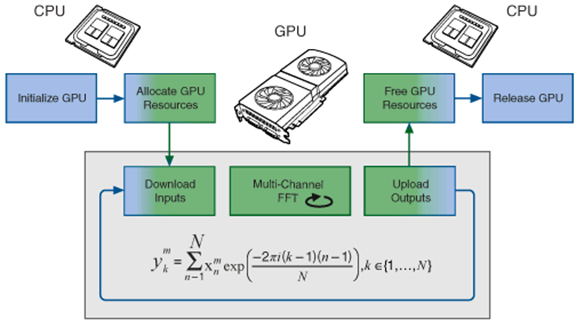
\includegraphics[scale=0.7]{images/gpuworkflow}
\caption{Exemple de calcul de la FFT sur GPU\protect\footnotemark}
\label{fig:gpgpu}
\end{figure}
\footnotetext{Source: \href{http://www.ni.com/white-paper/14077/fr/}{National Instruments}}


\chapter{État de l'art}

Intro

\section{PapARt}

\section{Système de réalité augmentée spatiale}

\section{Bilan}

\chapter{Développement d'application}

Comme présenté dans l'introduction (chapitre ~\ref{chap:intro}), le premier objectif du stage était le développement d'applications de réalité augmentée spatiale. Il était important, pour commencer, d'évaluer les possibilités mais aussi les contraintes qu'offrait le kit de développement. 
Ainsi, un travail d'analyse et de critique de l'interface de programmation (\emph{Application Programming Language API}) à été effectué en parallèle du développement d'applications.

\section{ReARTable}
\label{sec:reartable}
En tenant compte du contexte et du public ciblé par l'entreprise, il m'a paru intéressant de développer une démonstration dont le but était à la fois ludique et éducatif. J'ai donc choisi de recréer une Reactable\cite{reactable}, proposée par la société du même nom, en réalité augmentée spatiale, que nous avons nommé ReARTable.

La Reactable est un instrument de musique électronique permettant la génération de sons en direct, développé depuis 2003. Présenté sous la forme d'une table interactive, le son est généré via des éléments tangibles placés à sa surface Figure~\ref{fig:reactelem}. 

\begin{figure}[H]
\centering
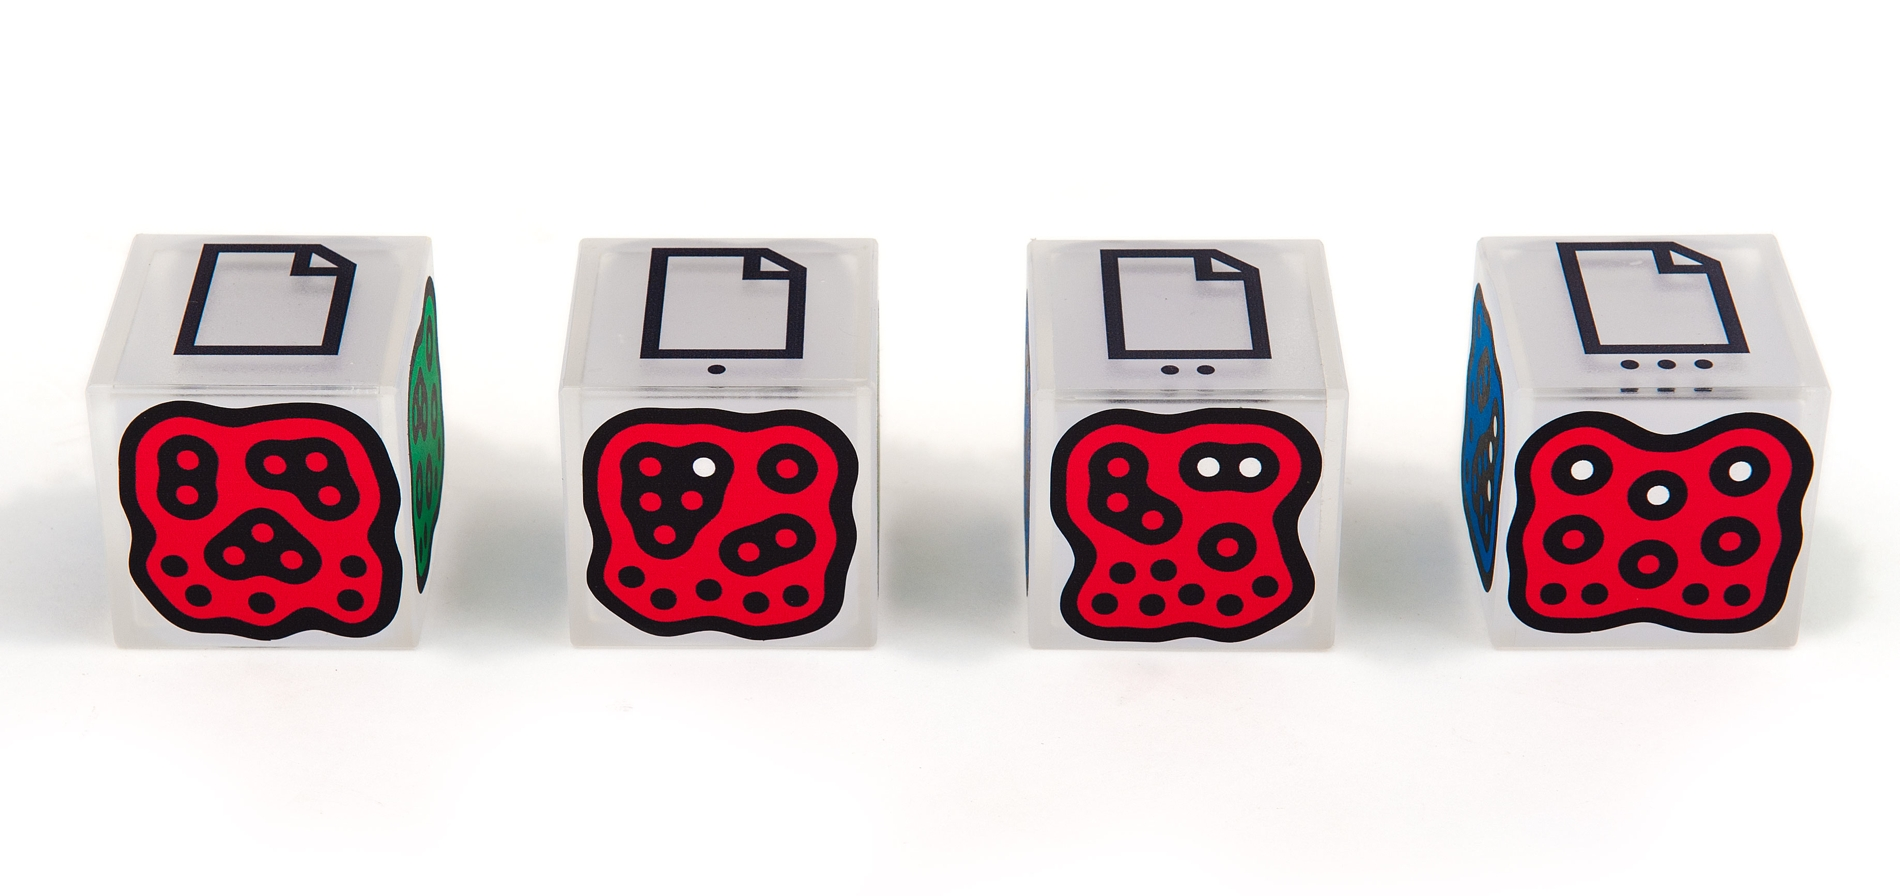
\includegraphics[width=0.6\textwidth]{images/reactelements}
\caption{Éléments tangibles utilisés pour la génération d'un élément de synthétiseur sur la Reactable\protect\footnotemark}
\label{fig:reactelem}
\end{figure}

\footnotetext{Source: \href{http://a-blok.com/FR/reactable.html}{Reactable : Elements tangibles}}

Chaque élément tangible représente un élément de synthétiseur qu'il est possible de contrôler de plusieurs façons:
\begin{itemize} 
\item La distance de l'élément par rapport à un autre élément. Cette propriété peut être utilisée pour contrôler, par exemple, l'interaction entre deux éléments.
\item L'orientation de l'élément sur la table. Cette propriété peut être utilisée pour contrôler, par exemple, la fréquence de l'élément ce qui va avoir pour effet si l'on prend l'exemple d'un battement de ralentir ou d'accélérer ce dernier.
\item La disposition de l'élément. Cette propriété permet, entre autres, de combiner des éléments pour créer de nouveaux sons, plus riches et plus complexes.
\item La position du doigt de l'utilisateur par rapport à un élément. On peut venir contrôler divers paramètres comme l'amplitude par exemple, en faisant graviter son doigt autour d'un élément.
\end{itemize}
Ainsi, c'est en combinant plusieurs éléments entre eux avec différentes orientations et différentes dispositions que l'utilisateur va pouvoir peu à peu "construire" sa musique.
Au-delà de la détection des éléments tangibles, la table est rétro éclairée et permet donc la visualisation, en direct, de la musique générée Figure~\ref{fig:reactivsu}.

\begin{figure}[H]
\centering
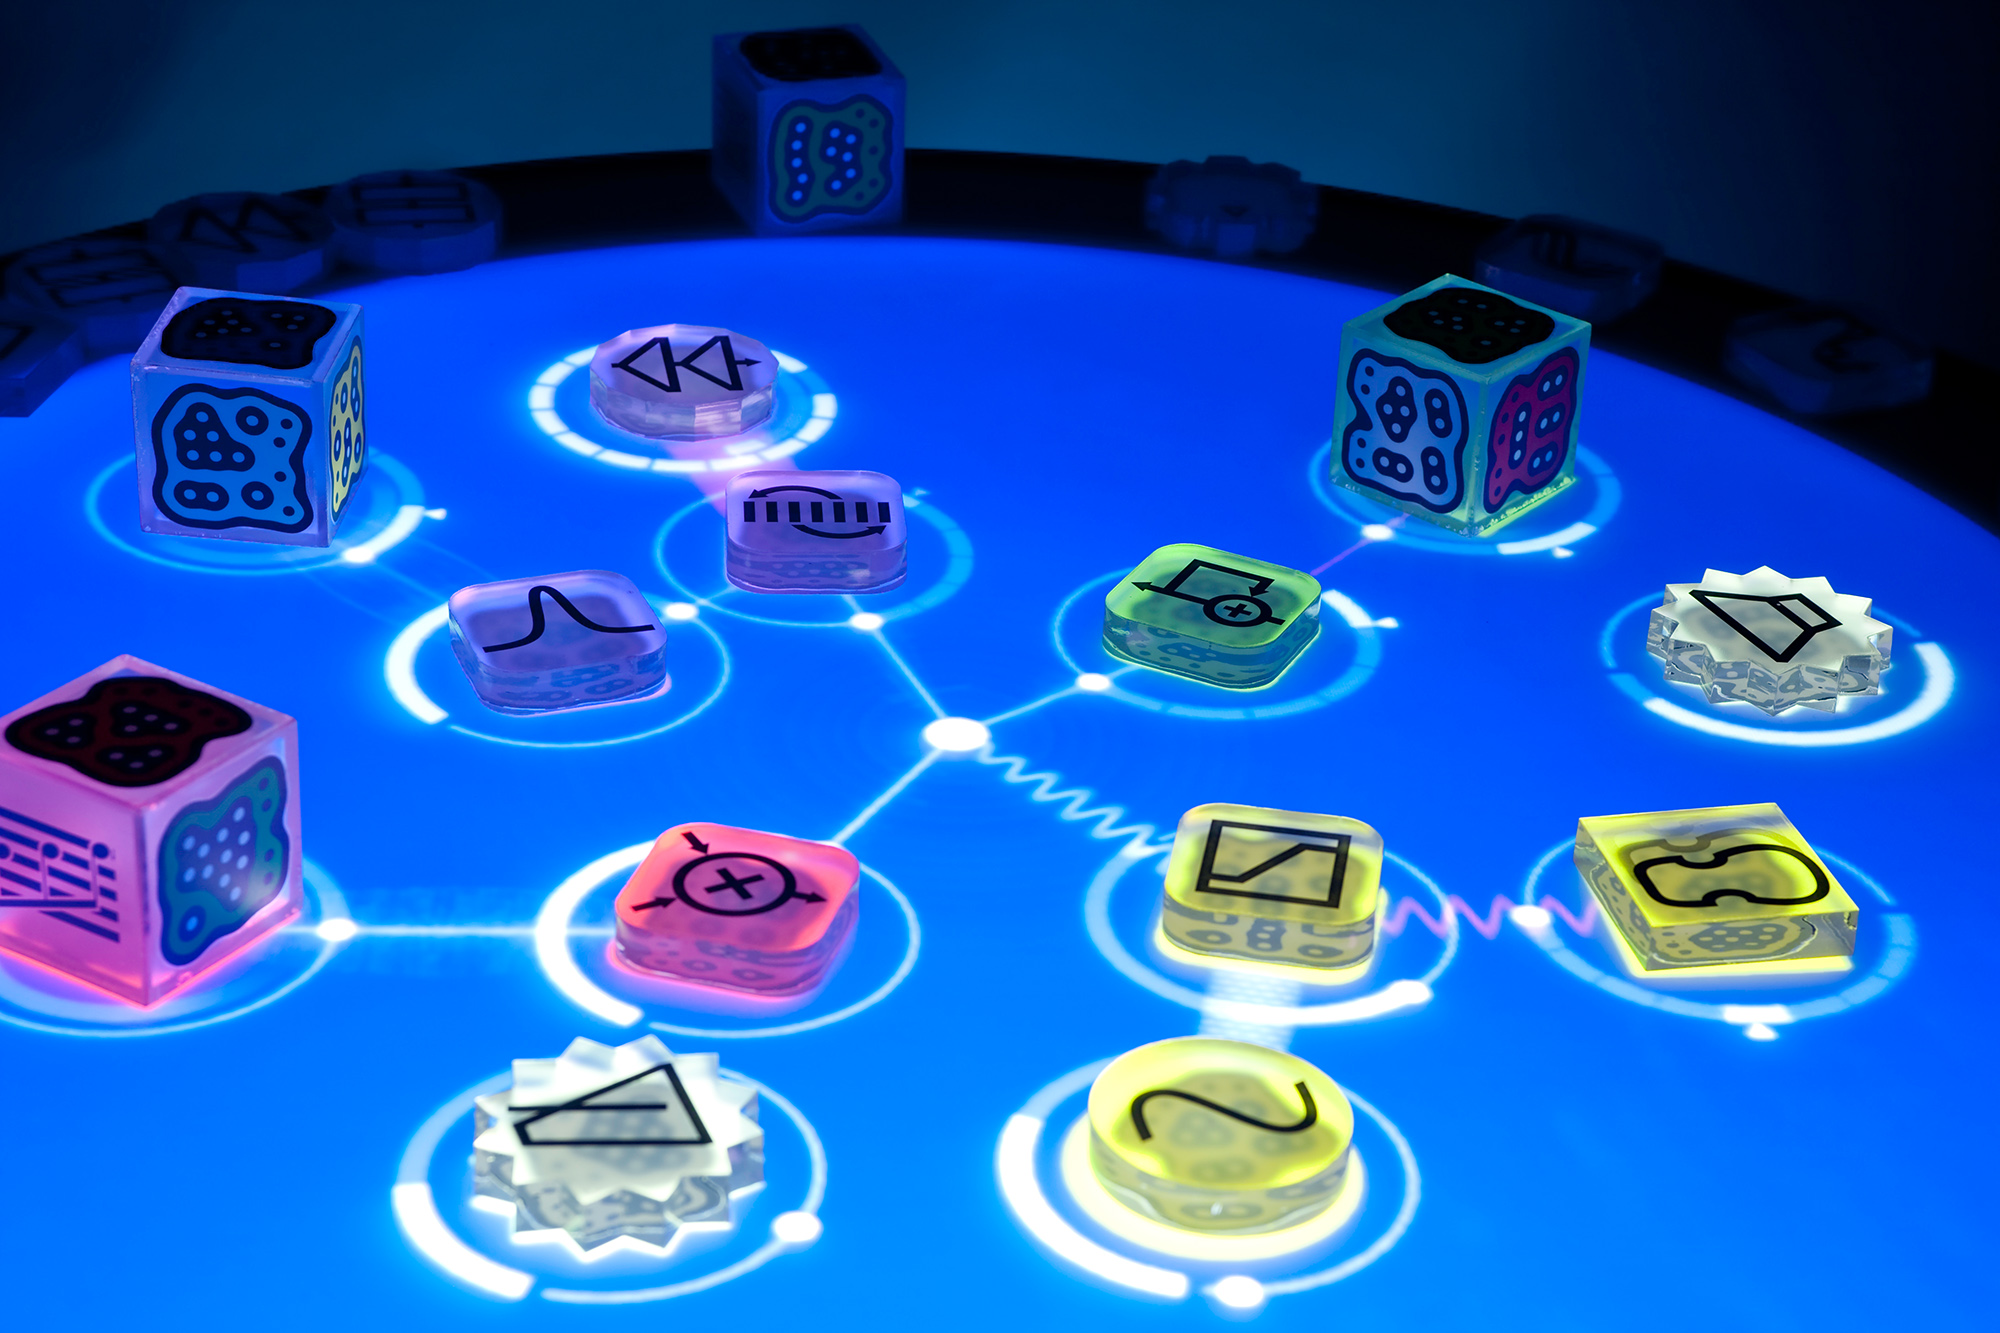
\includegraphics[width=0.65\textwidth]{images/reactvisu}
\caption{Visualisation du son sur la Reactable\protect\footnotemark}
\label{fig:reactivsu}
\end{figure}

\footnotetext{Source: \href{http://a-blok.com/FR/reactable.html}{Reactable}}

\subsection{Besoins de l'application}
\label{subsec:reartable:content}
Le but de l'application était de présenter une démonstration de ce qu'est capable de faire le système proposé par RealityTech, et non de créer un simulateur de musique en direct, finit, reprenant tous les points de la Reactable. Un tel développement pourrait faire l'objet d'un stage entier, ce qui n'était pas le cas ici.\\

Pour être en adéquation avec l'idéologie de l'entreprise, l'interface tangible ainsi que les modes d'interaction avec la musique étaient les points les plus importants à considérer. En gardant cela à l'esprit, nous avons défini les besoins fonctionnels principaux que voici :
\begin{itemize}
\item Générer du son en direct.
\item Créer une représentation physique du son. Chaque son ou élément sonore devait avoir une représentation physique qui lui était associée, c'est à dire, un élément ou groupement d'éléments tangibles le représentant.
\item Détecter des éléments physiques représentant les éléments sonores dans une image. L'application devait pouvoir détecter dans une image de caméra les divers éléments physiques présents, de façon à ce qu'ils soient utilisés pour identifier les éléments sonores.
\item Identifier les représentations des sons. Chaque élément sonore étant représenté par un ou plusieurs éléments physiques, l'application devait être capable, à partir des résultats de la détection, d'identifier et de différencier des éléments sonores entre eux. 
\item Modifier un élément sonore. L'application devait pouvoir contrôler certains paramètres définis à l'avance de chaque élément sonore généré. Ces paramètres ont pour but d'apporter à l'utilisateur un niveau de contrôle supérieur lors de la création de musique en direct.
\item Détecter des événements liés au toucher. Dans le cas du contrôle d'un son, l'utilisateur peut être amené à toucher des zones interactives pour déclencher divers effets.
\item Créer une visualisation basique d'un son. L'application devait proposer une visualisation du son généré, pour guider l'utilisateur dans son expérimentation.
\end{itemize}

\subsection{Choix et implémentation}
\label{subsec:reartable:impl}
L'application a donc été développée avec Processing, en utilisant, d'une part, PapARt pour la partie visualisation, détection et projection et, d'autre part, Sonic Pi\cite{sonicpi} pour la génération de musique en direct.
Sonic Pi est un synthétiseur temps réel qui permet de générer très facilement des sons de manière cohérente. Le gros avantage de Sonic Pi est qu'il résout tout seul bon nombre de problèmes posés par la génération dynamique de musique comme, par exemple, la synchronisation des boucles, les effets d'entrée et de sortie des instruments et bien d'autres, ce qui dé-complexifie énormément le processus.

Comme on peut le voir sur le schéma explicatif ci-dessous Figure~\ref{fig:reartable:generalscheme}, les éléments tangibles représentant des sons apparaissent sous forme de regroupement d'éléments ronds de petite taille (des aimants dans notre cas). L'idée derrière ce choix est d'encourager la manipulation d'éléments physiques pour garder le contenu numérique en contexte et ainsi favoriser la création. On peut différencier deux sons en fonction du contenu du regroupement (nombre, position et couleur des éléments regroupés).

\begin{figure}[H]
\centering
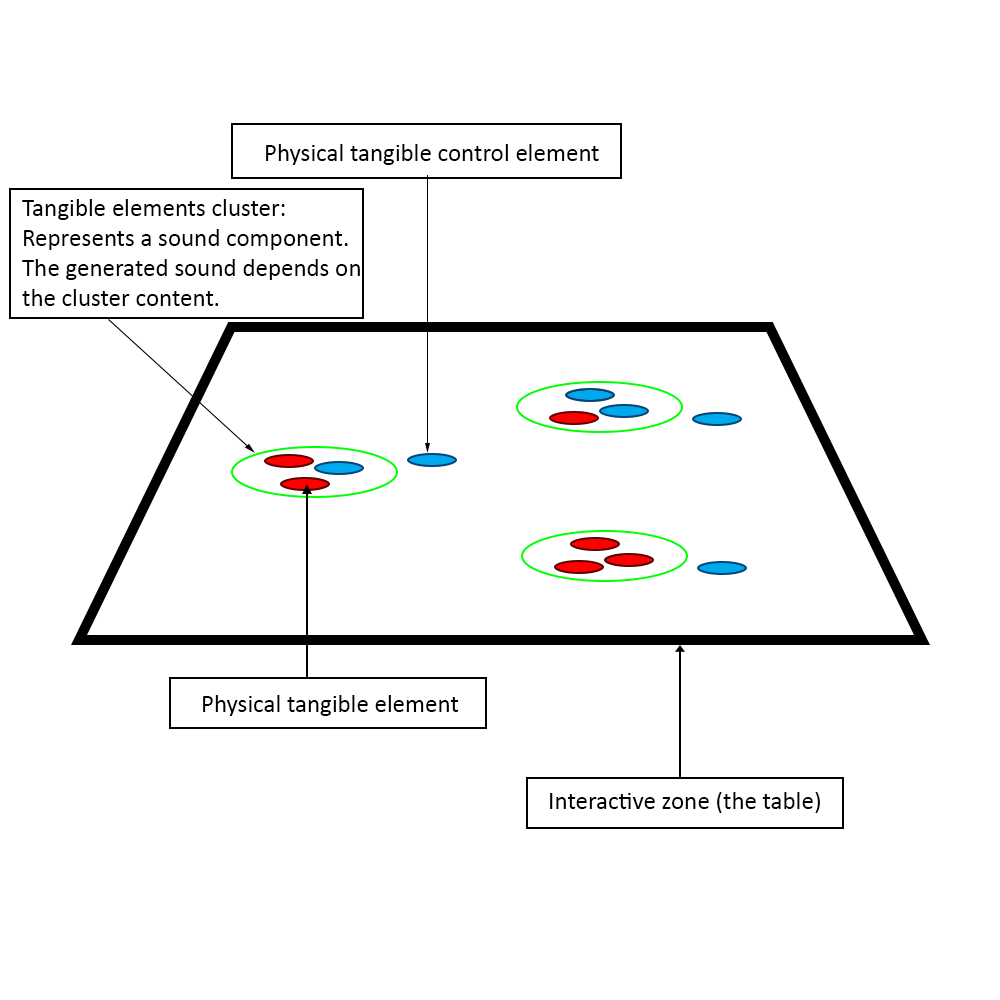
\includegraphics[width=0.5\linewidth]{images/rearproto}
\caption{ReARTable: Illustration du concept}
\label{fig:reartable:generalscheme}
\end{figure}

Une fois les éléments détectés, regroupés et identifiés, l'élément sonore associé peut être créé. La création de l'élément sonore se fait simplement via la transmission d'un message OSC\footnote{Le protocole OSC ou OpenSoundControl est un format de transmission de donnée conçu pour le contrôle en temps réel} à un serveur Sonic Pi préalablement démarré. Ce message contient l'identifiant unique de la boucle que Sonic Pi doit démarrer. Pour chaque élément sonore que l'application peut créer, Sonic Pi possède une fonction à exécuter que nous avons préalablement créée. Toutes les communications entre l'application et Sonic Pi utilisent ce protocole ce qui permet de démarrer/arrêter/modifier certaines parties du son en direct.

Pour ce qui est du contrôle du son, une zone autour du composant est définie dans laquelle soit un élément tangible, soit une interaction physique (avec le doigt) vont être détectés et convertis en interaction avec le contenu numérique Figure~\ref{fig:reartable:interactionzone}.

\begin{figure}[H]
\centering
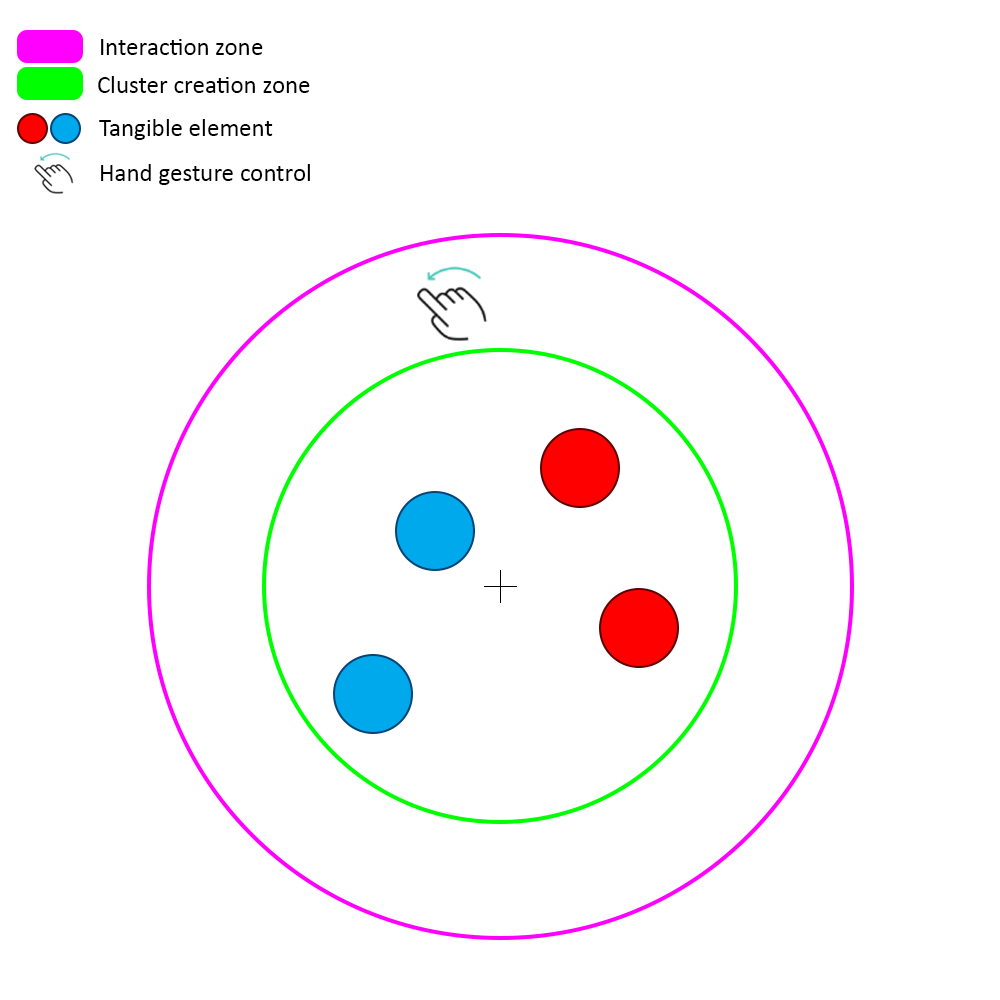
\includegraphics[width=0.45\textwidth]{images/reartable_cluster_interaction}
\caption{Schéma représentant la création d'un son avec zone d'interaction}
\label{fig:reartable:interactionzone}
\end{figure}

La dernière étape du développement de l'application concernait la visualisation de la musique générée section~\ref{subsec:reartable:content}. Cette étape n'a finalement pas été aboutie par manque de temps. L'idée était d'utiliser le spectre du son et les différentes fréquences qui le compose, récupérables à l'aide d'une transformée de Fourier\footnote{Opération mathématique permettant de décomposer un signal en la somme des signaux qui le compose \href{https://fr.wikipedia.org/wiki/Transformation_de_Fourier}{Wikipédia - Transformation de Fourier}.}, pour créer une visualisation globale basée sur les fréquences avec des variations visuelles en fonction de la hauteur, du tempo et de tous les autres paramètres du son qu'il est possible d'extraire et d'utiliser.\\

Vous trouverez Figure~\ref{fig:reartable:demo} un aperçu de l'état actuel de l'application. 

\begin{figure}[H]
\centering
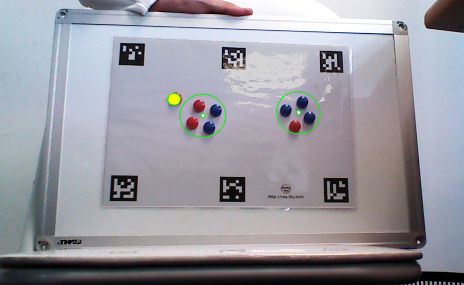
\includegraphics[width=0.65\linewidth]{images/reartable}
\caption{Démonstration de l'application}
\label{fig:reartable:demo}
\end{figure}

\newpage
\section{Extraction de document}
\label{sec:document}
Plus tard au cours de mon stage, nous avons eu l'occasion d'aborder des problématiques comme l'extraction et la numérisation de document (par exemple dans le cas de l'écriture d'une lettre en réalité augmentée) en tant que cas d'utilisation de PapARt. Il était donc opportun de développer une preuve de concept de cette fonctionnalité sous la forme d'une application de réalité augmentée spatiale.

Le but de ce développement était d'expérimenter diverses techniques de détection de document en temps réel, se basant ou non sur des connaissances à priori comme la taille du document, sa couleur, la couleur du fond (duquel il faudrait extraire le document), la présence d'éléments distinctifs (tels que des marqueurs fiduciaires ou des ronds colorés de petite taille) etc.

\subsection{Besoins de l'application}
\label{subsec:doc:content}
\begin{itemize}
\item Accéder au flux vidéo d'une caméra. L'application devait avoir access au flux vidéo d'une caméra filmant le document à détecter.
\item Détecter un document dans une image. Des images extraites du flux vidéo, l'application devait être capable, avec ou sans connaissance a priori, de détecter un document se trouvant dans cette image.
\item Extraire un document d'une image. Grâce au résultat de la détection, l'application devait être capable d'extraire ce document de l'image afin d'obtenir une image ne contenant que le dit document.
\end{itemize}

\subsection{Choix et implémentation}
\label{subsec:doc:impl}

La détection de document est un problème connu en traitement d'image, sur lequel j'avais déjà eu l'occasion de travailler lors de mon projet de fin d'études durant le deuxième semestre de mon année de Master 2.

Dans cette application, nous donc avons explorer plusieurs solutions sollicitant différents procédés dans le but d'essayer de trouver une solution adéquate à ce problème.

\subsubsection{Détection de document basée sur des marqueurs colorés} Le premier prototype de détection que nous avons conçu utilise beaucoup de connaissances à priori sur le document afin de faciliter la détection. Ainsi, le document cible est muni de lignes d'éléments ronds, colorés, de petite taille, dans un ou plusieurs de ses coins (fig~\ref{sub:doc}). Les éléments ronds de petite taille sont détectés grâce à PapARt en réalisant une convolution de l'image par un filtre permettant la détection de ces derniers dont le principe détaillé section~\ref{ssec:convtheo}.

Une fois les éléments détectés, ils sont regroupés en différentes lignes (fig~\ref{sub:docline}).
Une ligne est définie par un regroupement d'éléments dont l'écart entre chaque élément ne dépasse pas une certaine distance verticale ou horizontale. L'angle de la ligne est défini par les $x$ premiers éléments qui la compose, $x$ étant le nombre minimum d'éléments composant une ligne (fig~\ref{fig:doc:linecluster}). Si un autre élément "dérive" il est rejeté et la ligne est créée. Cette ligne est ensuite utilisée pour calculer deux vecteurs, dont un est confondu avec la ligne et le deuxième est perpendiculaire au premier (fig~\ref{sub:doclineperp}).

La détection finale du document se fait en calculant l'intersection des différents vecteurs verticaux et horizontaux (fig~\ref{sub:docextract})

\begin{figure}[H]
    \centering
	\subfloat[Document marqué à détecter]{
      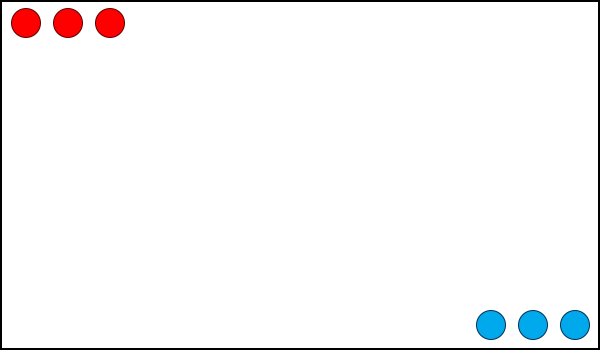
\includegraphics[width=0.45\textwidth]{images/document}
      \label{sub:doc}
      }
    \subfloat[Détection des éléments rond et création des lignes]{
      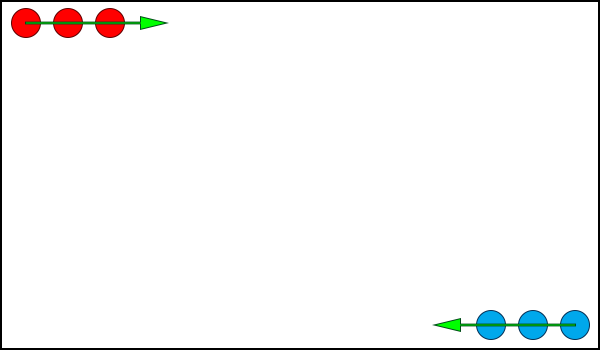
\includegraphics[width=0.45\textwidth]{images/doc-line}
      \label{sub:docline}
      }
      \\
      \subfloat[Génération des information manquante pour finaliser la détection]{
      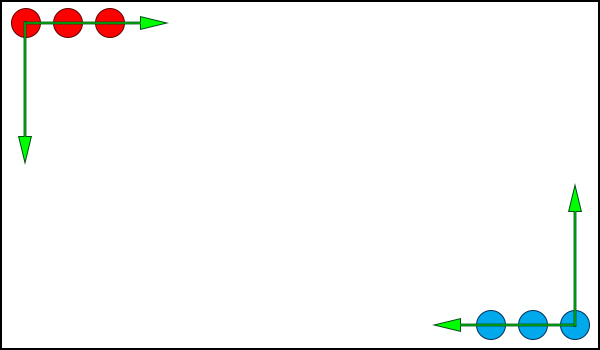
\includegraphics[width=0.45\textwidth]{images/doc-line-perp}
      \label{sub:doclineperp}
      }
    \subfloat[Document détecté]{
      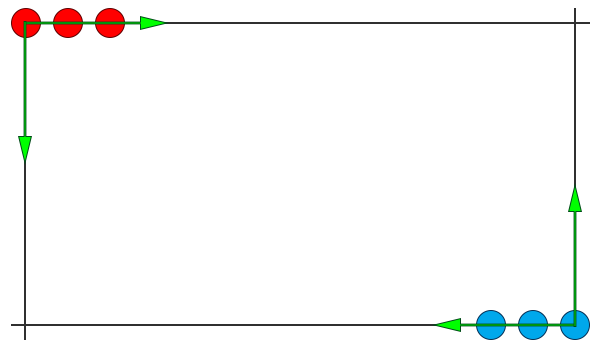
\includegraphics[width=0.45\textwidth]{images/doc-extraction}
      \label{sub:docextract}
      }
\caption{Détection de document étape par étape}
\label{fig:docdetection}
\end{figure}
	
\begin{figure}[H]
\centering
	\subfloat[]{
      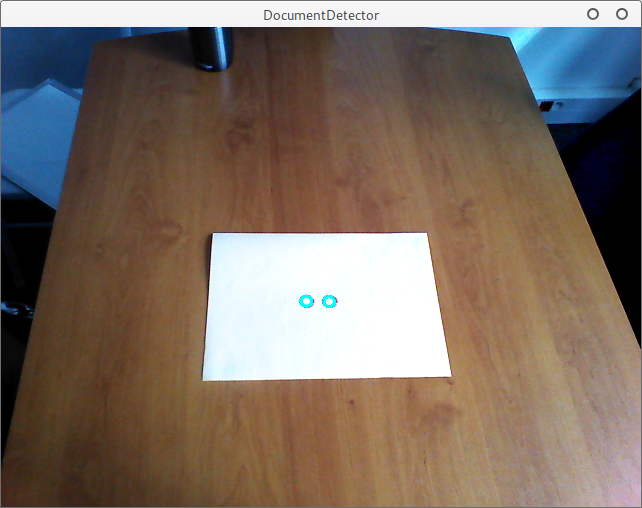
\includegraphics[width=0.45\textwidth]{images/document-detection-noline}
      \label{sub:doc:noline}
      }
      \subfloat[]{
      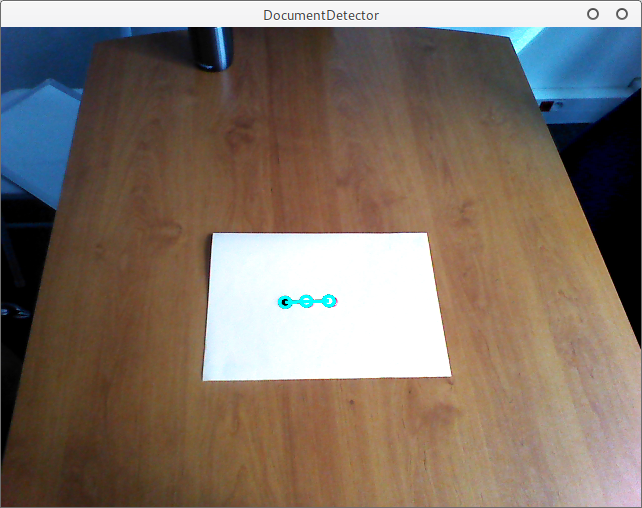
\includegraphics[width=0.45\textwidth]{images/document-detection-line}
      \label{sub:doc:line}
      }
      \caption{Détection et création d'une ligne a partir d'éléments colorés ($x = 3$)}
      \label{fig:doc:linecluster}
\end{figure}

Comme on peut le voir sur la figure ~\ref{sub:docextract}, lors de cette détection, les bords du document sont rognés. Généralement ces zones ne contiennent aucune information car elles correspondent le plus souvent aux marges verticales et horizontales présentes dans la plupart des documents. Cependant, comme évoqué dans les cas d'utilisation, cette détection ne sera pas seulement utilisée pour des documents de type A4, on pourra s'en servir comme outil pour suivre une feuille de papier à la manière des marqueurs \texttt{ARToolKitPlus}, ou pour détecter des post-it par exemple. Ainsi, ces marges ne peuvent pas être ignorées car elle sont susceptibles de contenir du contenu critique du document.

Une simple connaissance à priori de la distance des éléments ronds par rapport au coin permet de résoudre ce problème. Toutefois, si l'on souhaite obtenir une détection plus précise, il est conseiller d'utiliser des algorithmes de détection de contour couplés à des algorithmes d'extraction de lignes qui permettrons de retrouver de façon plus fidèle le coin du document. Cette re détection du coin est détaillée section~\ref{subsubsec:cannyhough}.

\subsubsection{Détection de document - Canny et transformée de Hough}
\label{subsubsec:cannyhough} 
Avec peu ou pas de connaissance a priori, la détection de document devient un problème compliqué et bien connu dans le domaine du traitement d'image surtout lorsqu'un besoin de temps réel vient s'ajouter à la tâche.

L'algorithme de Canny\cite{Canny86acomputational} est un filtre de détection de contours, permettant d'extraire d'une image (fig~\ref{sub:originalimage}) des contours très précis (fig ~\ref{sub:detectedge}) respectant trois critères : La bonne détection, la bonne localisation et la clarté de la réponse. Ces trois critères en font un très bon choix dans le cadre de la détection de document, où la qualité et surtout la précision de la détection est importante pour ne pas rogner des bouts de document par exemple. Cet algorithme a cependant tendance à laisser beaucoup de bruit issu de faibles contours tout de même détectés. C'est pourquoi il faut effectuer une étape de floutage préalable afin de lisser les zones à faibles contours.

Une fois les contours détectés, il est possible d'essayer d'extraire directement le document mais c'est une tâche complexe car elle requiert d'analyser les contours. Cette action peut être facilitée en utilisant une technique appelée transformée de Hough\cite{hough}. En effet, la transformée de Hough permet d'extraire n'importe quelle forme à partir d'une image contour en utilisant les propriétés mathématiques de celle ci. Dans notre cas, où nous souhaitons extraire des lignes droites, les propriétés mathématiques utilisées correspondent aux coordonnées polaires considérées comme plus robuste que l’équation de la droite (fig ~\ref{sub:detectline}). Il ne reste qu'à filtrer les lignes afin de trouver des potentiels documents dans une image.

\begin{figure}[H]
\centering
	\subfloat[Image originale]{
      
\includegraphics[width=0.45\textwidth]{images/detection-original-image}
      \label{sub:originalimage}
      }
      \\
	\subfloat[Canny - Détection de contours]{
      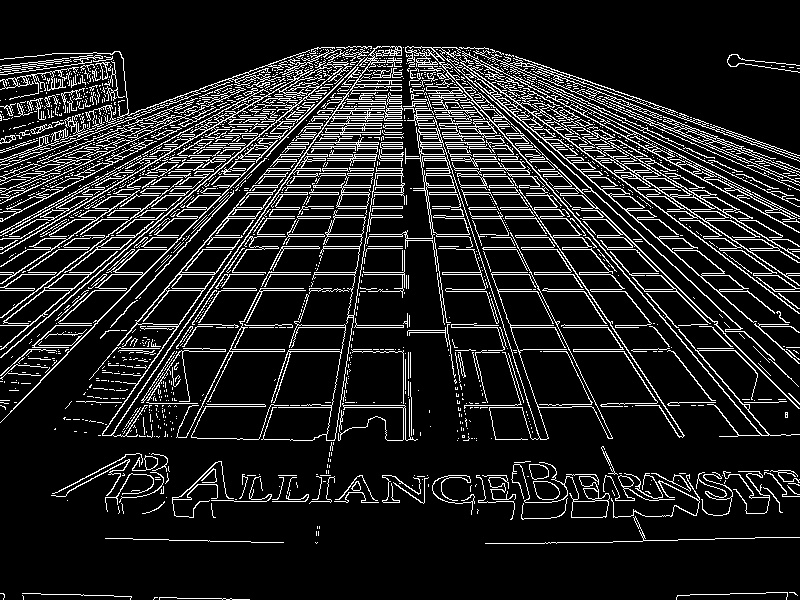
\includegraphics[width=0.45\textwidth]{images/cannysample}
      \label{sub:detectedge}
      }
    \subfloat[Transformée de Hough - Détection de lignes]{
      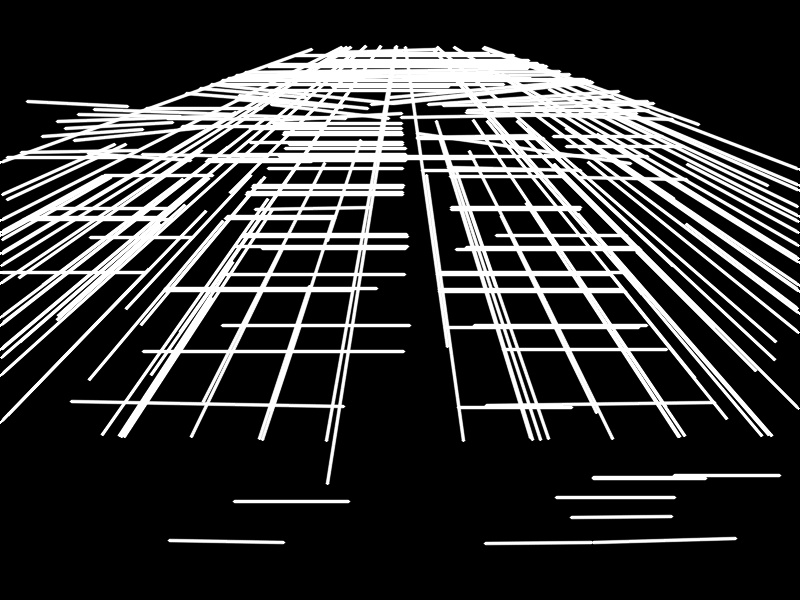
\includegraphics[width=0.45\textwidth]{images/houghsample}
      \label{sub:detectline}
      }
\caption{Détection de lignes : Canny + Hough\protect\footnotemark}
\label{fig:cannyhough}
\end{figure}
\footnotetext{Source : \href{http://funvision.blogspot.com/2016/01/hough-lines-and-canny-edge-sobel.html}{http://funvision.blogspot.com/2016/01/hough-lines-and-canny-edge-sobel.html}}

Cette succession de traitements est cependant lourde et peut difficilement être effectuée en temps réel sur des images haute résolution. 

Dans notre cas, nous nous somme servis de ces deux algorithmes mais uniquement sur des parties d'image (de petite résolution) de façon à améliorer une première détection grossière effectuée notamment à l'aide de marqueurs colorés. Une fois la première détection effectuée, nous obtenons une position plus ou moins précise des quatre coins nécessaires à l'extraction du document. Nous utilisons cette information sur la position potentielle des coins pour extraire des sous-images centrées sur ces coins (fig. ~\ref{sub:subimage:subimage}) que nous seuillons afin d'obtenir une image binaire Figure~\ref{sub:subimage:tresh}. Ensuite, nous appliquons les deux algorithmes mentionnés plus tôt, à savoir la détection de contours (fig. ~\ref{sub:subimage:canny}) puis la détection de lignes (fig. ~\ref{sub:subimage:hough}). Après cela, nous filtrons le résultat de la détection de ligne pour obtenir exactement une ligne verticale et une ligne horizontale. Une fois ces deux lignes trouvées, nous calculons les équations de droite (pente et constante) associées, pour pouvoir en calculer l'intersection et ainsi trouver le coin dans notre sous image (fig ~\ref{sub:subimage:corner}).

\begin{figure}[H]
\centering
	\subfloat[Sous image autour d'un coin.]{
      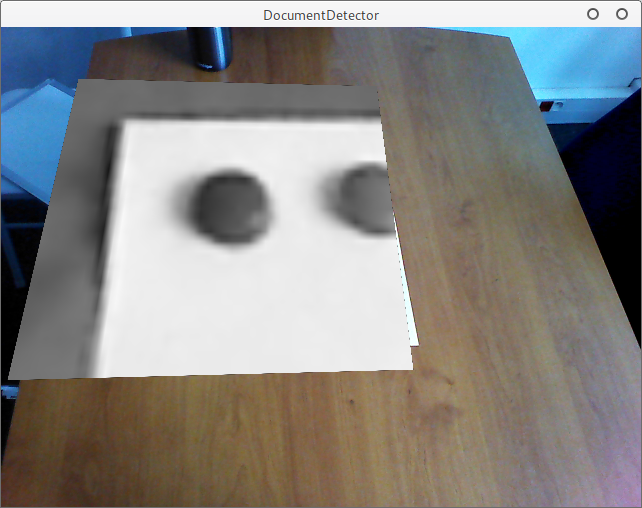
\includegraphics[width=0.33\textwidth]{images/doc-original}
      \label{sub:subimage:subimage}
      }\\
      \subfloat[Seuillage de l'image originale]{
      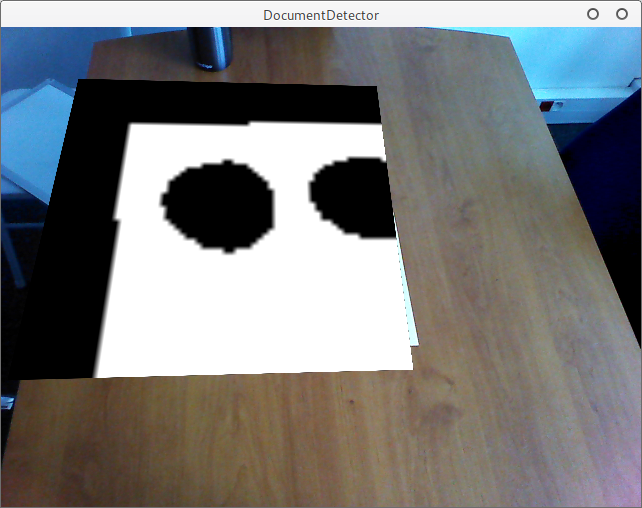
\includegraphics[width=0.33\textwidth]{images/doc-tresh}
      \label{sub:subimage:tresh}
      }
    \subfloat[Canny - Détection de contour basée sur un seuillage de l'image originale]{
      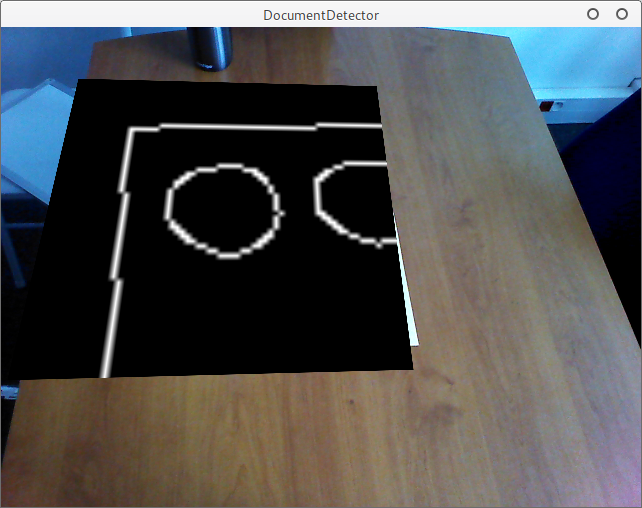
\includegraphics[width=0.33\textwidth]{images/doc-canny}
      \label{sub:subimage:canny}
      }
      \\
	\subfloat[Hough - Détection de lignes basée sur le résultat de Canny]{
      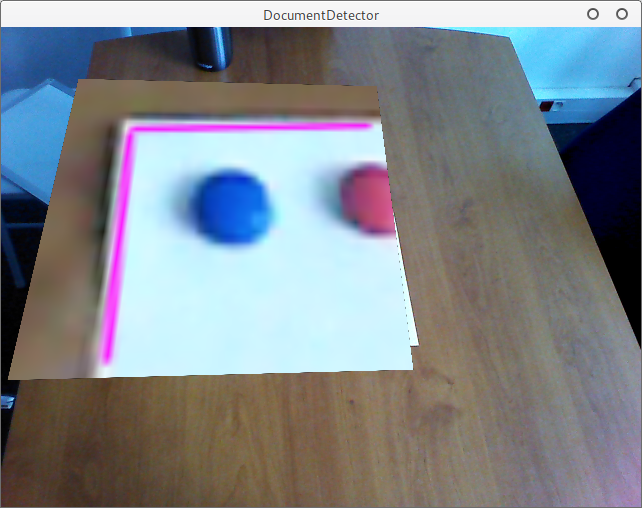
\includegraphics[width=0.33\textwidth]{images/doc-hough}
      \label{sub:subimage:hough}
      }
    \subfloat[Détection finale du coin.]{
      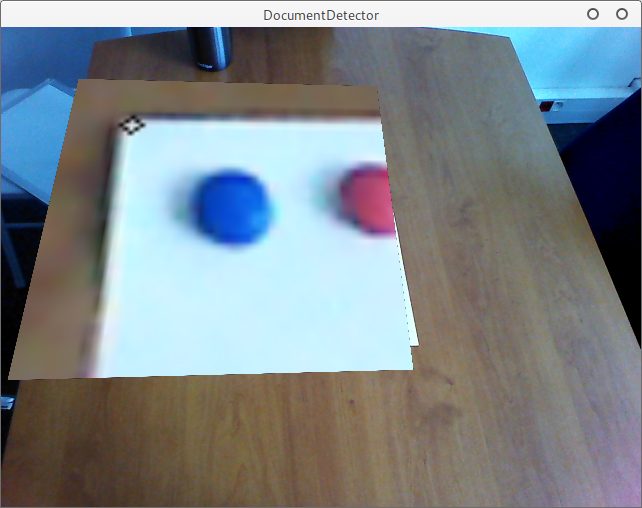
\includegraphics[width=0.33\textwidth]{images/doc-corner}
      \label{sub:subimage:corner}
      }
\caption{Affinage de la détection d'un coin du document}
\label{fig:corner-redetect}
\end{figure}

\subsection{Bilan}
\label{subsec:doc:bilan}
Pour finir, un comparatif des différents résultats obtenus est présenté sur la Figure~\ref{fig:docdetect:results}.
On peut observer quelques points notables : En utilisant Canny puis Hough pour améliorer la détection d'un coin, l'extraction est plus fidèle au document réel Figure~\ref{sub:docdetect:corner} et ~\ref{sub:docdetect:double-corner}. En effet, les coins détectés sont plus précis qu'avec des hypothèses effectuées à priori Figure~\ref{sub:docdetect:simple} et~\ref{sub:docdetect:double}. Toutefois, cette méthode est moins rapide car elle requiert de nombreux calculs supplémentaires. Lorsque utilisée en temps réel, une détection avec connaissance à priori du modèle sera bien plus robuste, car elle ne dépend pas d'une deuxième détection qui à beaucoup de chance d'échouer (seuillage, détection de contours, détection de lignes, intersection entre deux droites puis obtention finale du coin). Ainsi, la méthode à utiliser variera avec les cas d'utilisation. Par exemple, dans le cadre d'une application de scan de document, une méthode d'extraction de document plus précise sera envisagée, mais pour une estimation de pose et un suivi de document il sera préférable d'utiliser une détection plus rapide et robuste.

\begin{figure}[H]
\subfloat[Avec connaissance à priori: Taille du document et distance élément $\longleftrightarrow$ coin]{
      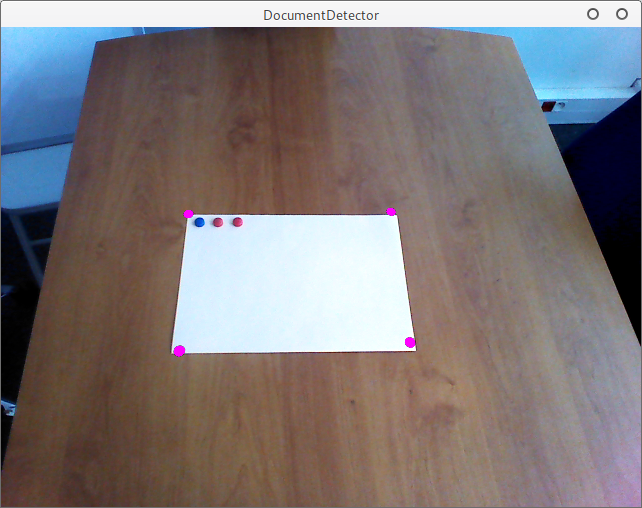
\includegraphics[width=0.5\textwidth]{images/document-detection-simple}
      \label{sub:docdetect:simple}
      }
      \subfloat[Avec connaissance à priori: Taille du document et distance élément $\longleftrightarrow$ coin]{
      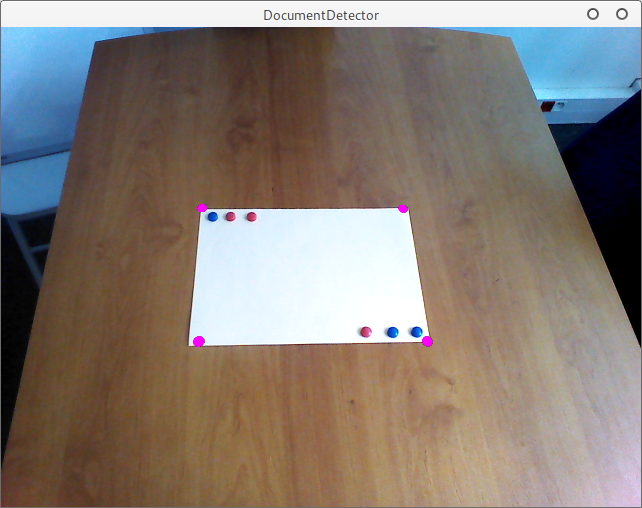
\includegraphics[width=0.5\textwidth]{images/document-detection-double}
      \label{sub:docdetect:double}
      }\\
      \subfloat[Avec connaissance à priori: Taille du document]{
      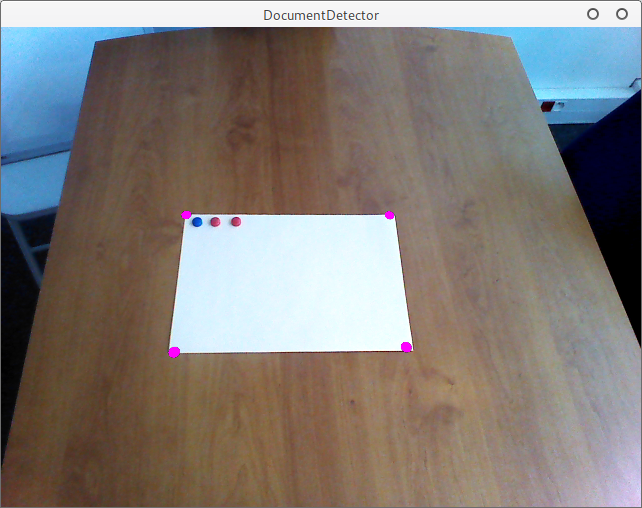
\includegraphics[width=0.5\textwidth]{images/document-detection-corner}
      \label{sub:docdetect:corner}
      }
      \subfloat[Sans connaissance à priori]{
      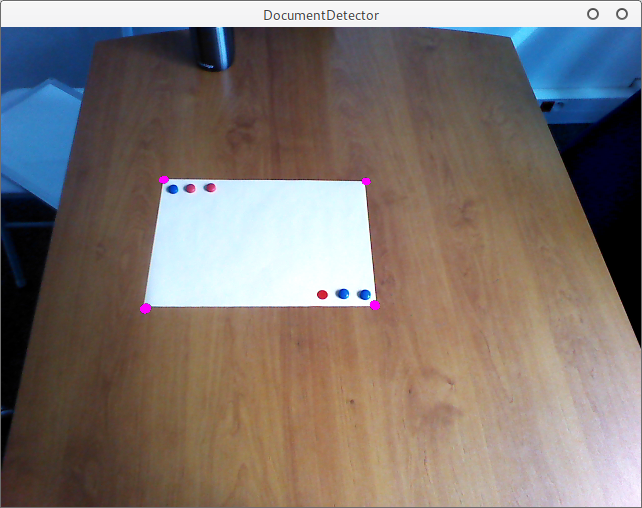
\includegraphics[width=0.5\textwidth]{images/document-detection-double-corner}
      \label{sub:docdetect:double-corner}
      }
      \caption{Résultats des différentes versions de la détection de document.}
      \label{fig:docdetect:results}
\end{figure}


%Ne pas numéroter cette partie
\part*{Annexes}
%Rajouter la ligne "Annexes" dans le sommaire
\addcontentsline{toc}{part}{Annexes}

\chapter*{Annexe 1}
\addcontentsline{toc}{chapter}{Annexe 1}

%changer le format des sections, subsections pour apparaittre sans le num de chapitre
\makeatletter
\renewcommand{\thesection}{\@arabic\c@section}
\makeatother

%recommencer la numérotation des section à "1"
\setcounter{section}{0}

Intro

\section{Partie 1}

Bla

\subsection{Sous-partie 1}

Bla

\subsection{Sous-partie 2}

Bla

\subsection{Sous-partie 3}

Bla

\section{Partie 2}

Bla

\subsection{Sous-partie 1}

Bla

\subsection{Sous-partie 2}

Bla

\subsection{Sous-partie 3}

Bla

\chapter*{Annexe 2}
\addcontentsline{toc}{chapter}{Annexe 2}

%recommencer la numérotation des section à "1"
\setcounter{section}{0}

Intro

\section*{Prérequis}
\addcontentsline{toc}{section}{Prérequis}

Bla

\begin{itemize}
\item item1;
\item item2;
\item item3;
\item item4.
\end{itemize}

Bla

\section{Partie 1}

Bla

\subsection{Sous-parie 1}

Bla

\subsection{Sous-parie 2}

Bla

\section{Partie 2}

\begin{center}
\textsc{Attention !}

\textit{Texte d'avertissement}
\end{center}

Bla

\newpage

\section{Partie 3}

Bla

\begin{figure}[!ht]
\begin{center}
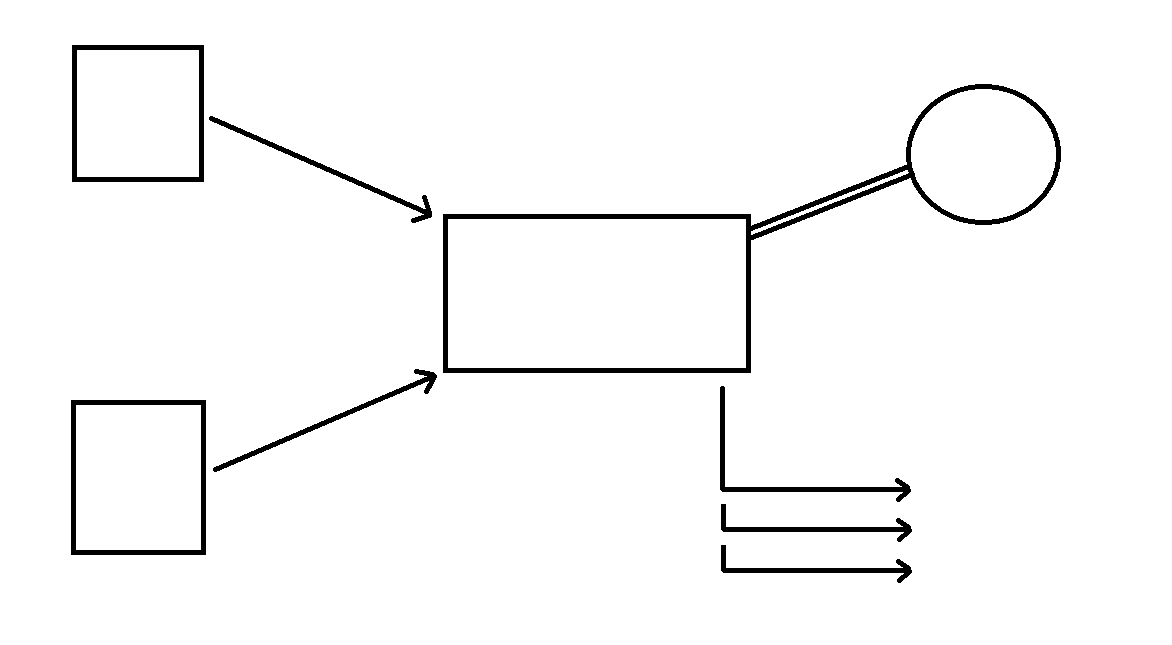
\includegraphics[height=8cm]{presentation/schema}
\end{center}
\caption[schema]{Presentation schema}
\end{figure}

\paragraph*{Paragraphe 1}
~\\
\hskip7mm

Bla

\paragraph*{Paragraphe 2}
~\\
\hskip7mm

Bla

\paragraph*{Paragraphe 3}
~\\
\hskip7mm

Bla

\chapter*{Annexe 3 - Unity diagramme d'exécution des fonctions}
\addcontentsline{toc}{chapter}{Annexe 3 - Unity diagramme d'exécution des fonctions}
\label{annexe:unity}

\begin{figure}
\centering
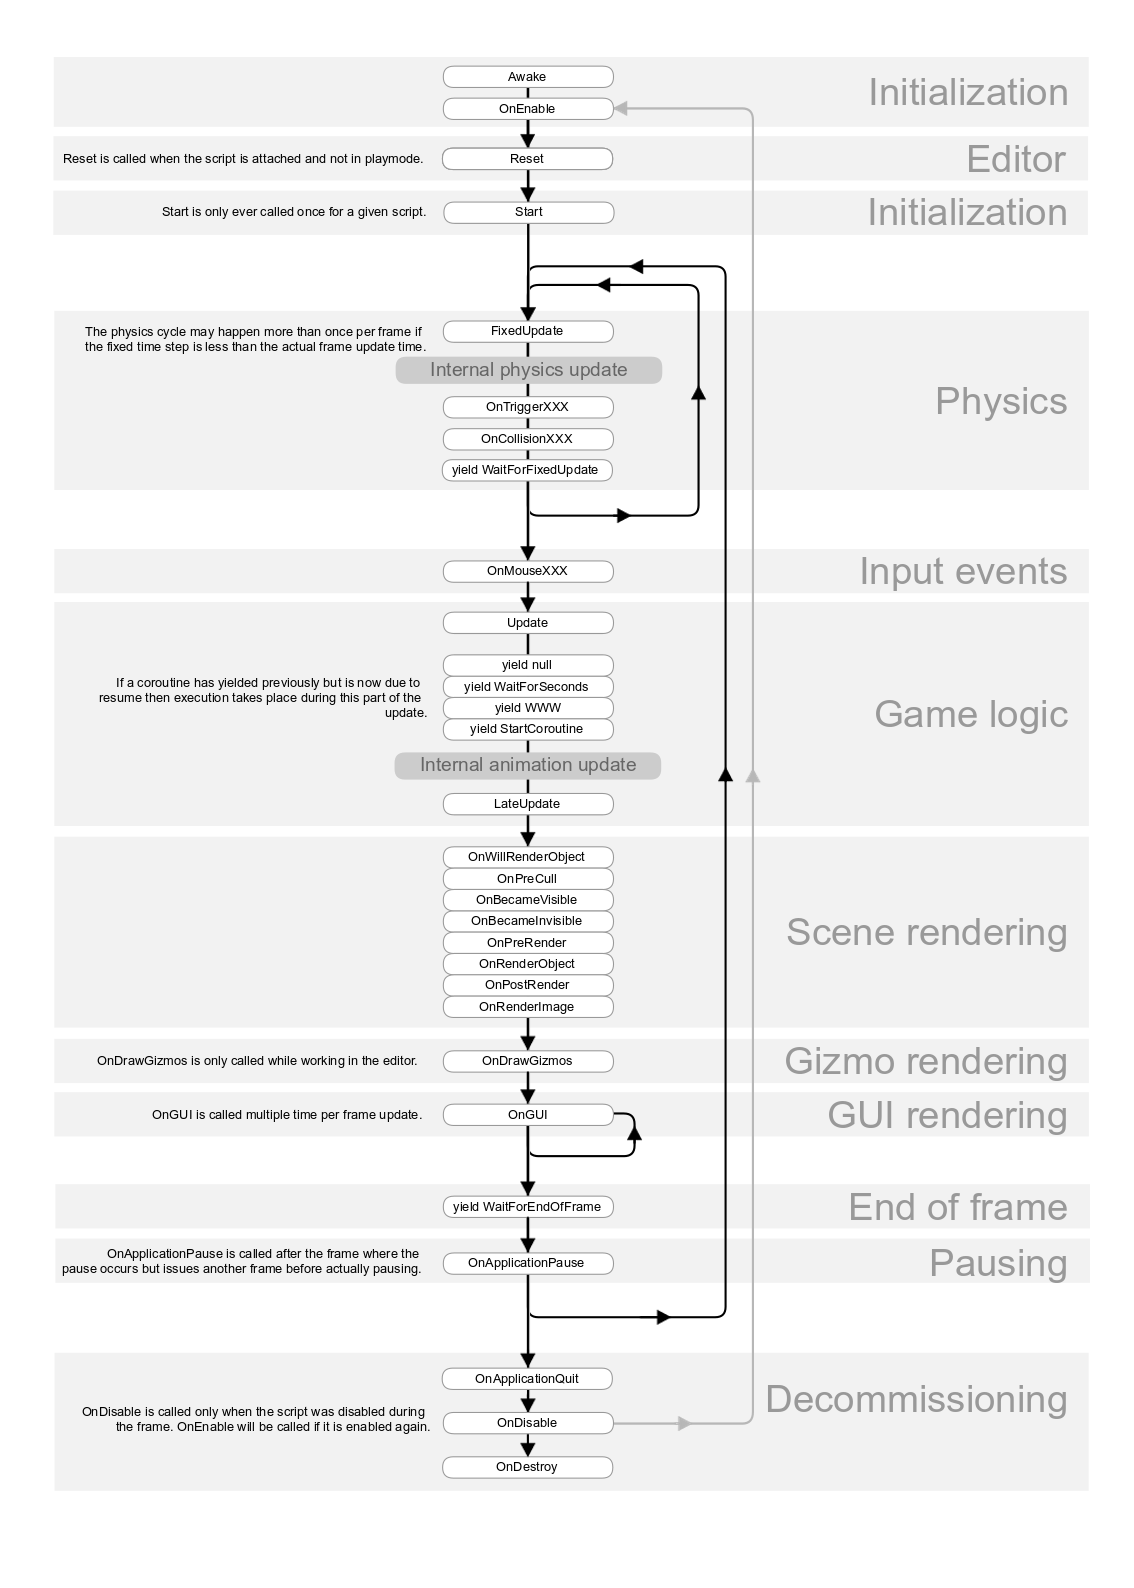
\includegraphics[width=\linewidth]{images/monobehaviour_flowchart}
\end{figure}

\newpage

%récupérer les citation avec "/footnotemark"
\nocite{*}

%choix du style de la biblio
\bibliographystyle{plain}
%inclusion de la biblio
\bibliography{bibliographie.bib}
%voir wiki pour plus d'information sur la syntaxe des entrées d'une bibliographie

\end{document}